% Historical proof exposition, retained as source but not included in paper.tex.
% Current implementation-facing statements are in theory_current.tex.
\newpage
\appendix
\onecolumn
\section{Portfolio Configuration Specification}
\label{app:operators}
\begin{table}[ht]
\centering\small
\caption{The 18 allocation slots of the BAMOR update portfolio across coverage
(C), recovery (R) and extreme-preference (E) families. Relabel denotes the
fraction of the replay minibatch assigned fresh preferences; $C_o$ counts total
preference copies per batch; $K_o^Q$ and $K_o^\pi$ are critic and actor
candidate counts; $\lambda_o$ and $b_o$ weight vector-target and
behavior-cloning losses.}
\label{tab:operators}
\begin{tabular}{llrrrrrr}
\toprule
Slot & Sampler & Relabel & $C_o$ & $K_o^Q$ & $K_o^\pi$ & $\lambda_o$ & $b_o$\\
\midrule
C1 & edge & 1 & 3 & 1 & 1 & 0.05 & 0 \\
C2 & stratified & 1 & 2 & 1 & 1 & 0.05 & 0 \\
C3 & mixed & 1 & 2 & 1 & 1 & 0.05 & 0 \\
C4 & edge & 1 & 3 & 4 & 1 & 0.05 & 0 \\
C5 & stratified & 1 & 3 & 4 & 1 & 0.05 & 0 \\
C6 & mixed & 1 & 3 & 4 & 1 & 0.05 & 0 \\
C7 & edge & 1 & 3 & 4 & 3 & 0.05 & 0.006 \\
\midrule
R1 & mixed & 1 & 2 & 1 & 1 & 0.05 & 0 \\
R2 & stratified & 1 & 3 & 4 & 1 & 0.05 & 0 \\
R3 & mixed & 1 & 3 & 4 & 1 & 0.05 & 0 \\
R4 & mixed & 1 & 2 & 1 & 4 & 0.05 & 0 \\
R5 & uniform & 1 & 3 & 4 & 4 & 0.05 & 0 \\
R6 & stratified & 1 & 3 & 4 & 4 & 0.05 & 0 \\
R7 & mixed & 1 & 3 & 4 & 4 & 0.05 & 0.01 \\
\midrule
E1 & edge & 1 & 3 & 5 & 5 & 0.06 & 0 \\
E2 & edge & 0 & 1 & 5 & 5 & 0.06 & 0 \\
E3 & edge & 1 & 3 & 5 & 5 & 0.06 & 0.004 \\
E4 & edge & 1 & 3 & 5 & 5 & 0.06 & 0 \\
\bottomrule
\end{tabular}
\end{table}

Following the initial 5,000-step initialization phase, the first ten
1,500-step blocks follow the deterministic coverage schedule:
C6, C1, C2, R1, R5, E1, E2, E3, C7, R7.

The 18 slots specify 14 distinct parameter settings. The pairs C3/R1; C5/R2; C6/R3; E1/E4 share settings and keep separate scores and counts. For three objectives, C4 also coincides with C5 and R2, giving 13 distinct behaviors.

\clearpage
\section{Historical Experiments}
\label{app:historical_synthetic}

\subsection{Experimental setup}
\label{sec:exp_setup}

\textbf{Environment.}  A 1-D continuous navigation task with position $p\in[-10,10]$ and velocity action $a\in[-1,1]$.  The reward vector is 2-dimensional, $\mathbf{r}=(r_{\text{safety}}, r_{\text{progress}})$, constructed so that \emph{each mode collapses one objective to a different state feature}: in ``safety'' mode $r_{\text{safety}}$ is position-responsive while $r_{\text{progress}}$ collapses to the action; in ``progress'' mode the roles reverse; in ``balanced'' mode both are position-responsive.  This creates different mode-specific return geometries; all simplex preferences remain valid scalarized utilities.  Three modes cycle deterministically every \texttt{switch\_interval}$=300$ steps with ground-truth anchors $w_0{=}[0.85,0.15]$ (safety-dominated), $w_1{=}[0.15,0.85]$ (progress-dominated), $w_2{=}[0.5,0.5]$ (balanced).

\textbf{Algorithms.}  We compare five methods, all sharing the same actor--critic backbone and weight-conditioned policy $\pi(a\mid s, w)$; they differ \emph{only} in how preference weights are sampled and whether the cone estimator is active:
\begin{itemize}[topsep=1pt,leftmargin=1.3em]
    \item \textbf{BAMOR-TC}: Target Cone with frozen-uniform belief. Cone statistics $\hat w_{\mathrm{anchor}}$ are estimated from reward variance; $w \sim \mathrm{Dir}(\kappa \cdot \tilde w)$ with $\kappa{=}20$. No online mode-change detector.
    \item \textbf{BAMOR $+$ surprise}: BAMOR-TC with the Mahalanobis online change-point detector active (threshold$=7$, cooldown$=290$ steps, warm-up$=150$).
    \item \textbf{BAMOR $-$ Cone}: historical ablation retaining the surprise detector while disabling the cone. The current implementation uses $\mathrm{Dir}(\mathbf 1)$; the historical output files do not record the sampler concentration.
    \item \textbf{Uniform-sampling}: $w \sim \mathrm{Dir}(\mathbf{1})$ every step, no cone, no belief---a preference-conditioned actor--critic baseline.
    \item \textbf{Fixed-weight}: $w=[0.5,0.5]$ throughout training, no cone, no belief---a scalar sanity baseline.
\end{itemize}
All methods train for $100{,}000$ environment steps with identical network sizes, learning rates, replay buffers, and a 20-seed sweep on a shared GPU cluster.  Final performance is measured by hypervolume (HV) against reference point $(-5,-5)$, evaluated (i) globally over a dense grid of $21$ preference weights under the mode-switching schedule and (ii) per mode by locking the environment to a fixed mode and re-evaluating on $11$ weights.

% ── 6.2 Main result ─────────────────────────────────────────────────────────
\subsection{Historical synthetic results}

\begin{table}[t]
\centering\small
\caption{Hypervolume (HV) on the synthetic non-stationary MO environment at 100K steps (5 seeds).  Mode anchors are $w_0{=}[0.85,0.15]$, $w_1{=}[0.15,0.85]$, $w_2{=}[0.5,0.5]$.  Reference point $(-5,-5)$.  Bold = best per column; BAMOR dominates Mode~1 (skewed cone, $+28.2\%$ over Uniform) and wins on three of four columns.}
\label{tab:main_results}
\begin{tabular}{lcccc}
\toprule
Method & HV overall & HV Mode 0 & HV Mode 1 & HV Mode 2 \\
\midrule
BAMOR (full) & $130.9{\pm}16.9$ & \textbf{$21.9{\pm}0.4$} & \textbf{$48.2{\pm}2.4$} & \textbf{$125.5{\pm}27.7$} \\
BAMOR$-$Cone & \textbf{$136.0{\pm}17.1$} & $19.8{\pm}2.7$ & $42.7{\pm}6.5$ & $124.7{\pm}24.9$ \\
BAMOR$-$Surprise & $115.2{\pm}39.6$ & $21.6{\pm}0.6$ & $36.0{\pm}8.3$ & $109.5{\pm}45.0$ \\
Uniform-sampling & $122.3{\pm}54.8$ & $21.1{\pm}1.3$ & $37.6{\pm}18.3$ & $119.4{\pm}55.9$ \\
Fixed-weight & $117.2{\pm}39.4$ & $14.3{\pm}6.2$ & $34.1{\pm}5.6$ & $102.4{\pm}40.1$ \\
\bottomrule
\multicolumn{5}{l}{\footnotesize HV values in units of $10^3$; $\pm$ = one standard deviation across 5 seeds.}
\end{tabular}
\end{table}

BAMOR-TC had higher sample-mean HV than Uniform in all four reported columns. Overall means were $136.2\times10^3$ and $121.1\times10^3$, respectively, with standard deviations $23.6\times10^3$ and $50.5\times10^3$. Across paired seeds, BAMOR-TC won 12/20 overall comparisons; a two-sided Wilcoxon signed-rank test gave $p=0.4749$. Per-mode tests gave $p=0.6215$, $0.7841$, and $0.8124$. The sample-mean differences therefore do not establish a reproducible advantage over uniform sampling.

\subsection{Historical ablations}
\label{sec:exp_ablation}

The surprise-enabled and no-cone variants had lower observed mean overall HV than BAMOR-TC, by approximately $29\%$ and $28\%$. These observations motivate retaining the simpler frozen-belief synthetic variant. Comparing BAMOR-TC directly with the no-cone variant changes both the cone and surprise configuration, so it does not isolate the cone effect. The archived metadata also do not fully identify the historical no-cone sampler configuration. The negative results remain part of the record.

% ── 6.4 Qualitative% ── 6.4 Qualitative: per-mode Pareto arcs ───────────────────────────────────
\subsection{Per-mode Pareto fronts: visualising the piecewise sub-manifolds}

\begin{figure}[t]
\centering
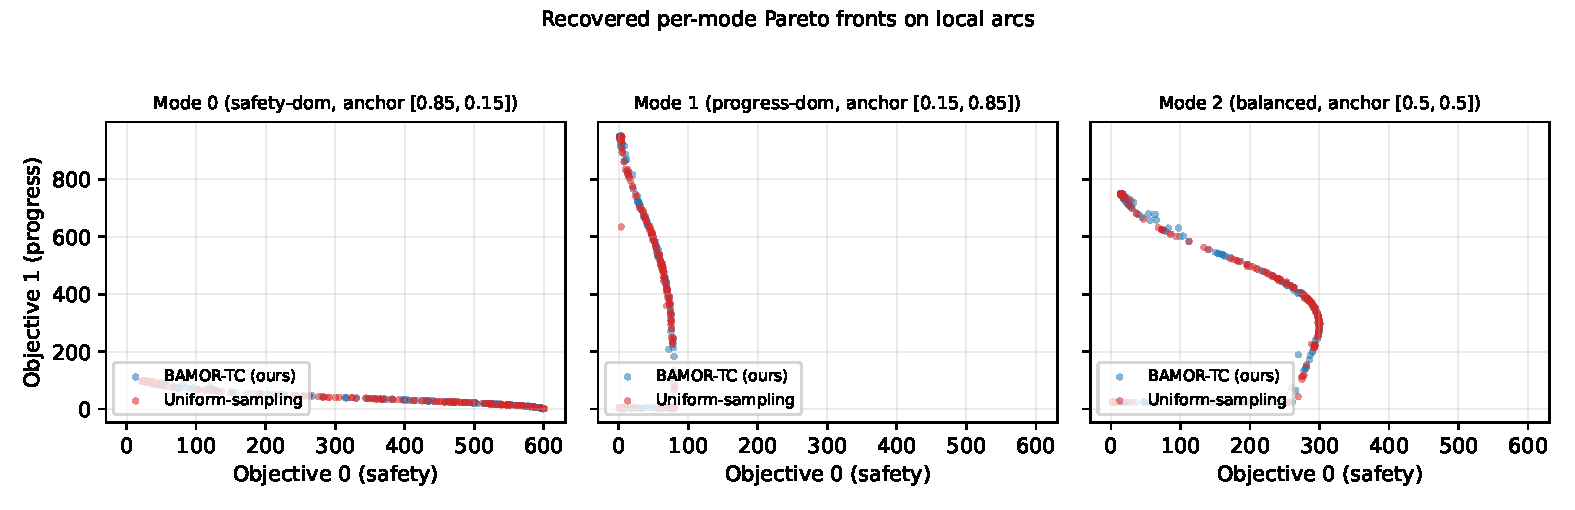
\includegraphics[width=0.98\linewidth]{fig_pareto_permode.pdf}
\caption{Per-mode Pareto fronts recovered by BAMOR-TC and Uniform, pooled across seeds and weights in the evaluation grid. Mode~0's front is a near-horizontal arc (progress capped), Mode~1's is near-vertical (safety capped), and Mode~2 is a full elbow. Both methods recover the same mode-wise geometry, while Uniform shows more low-return scatter in several panels.}
\label{fig:pareto_permode}
\end{figure}

Fig.~\ref{fig:pareto_permode} illustrates the different return geometries of the three synthetic modes. These are separate mode-conditioned fronts; their union is not the Pareto front of a single common evaluation task.  The substrate caps in Modes~0 and~1 appear as near-horizontal and near-vertical arcs respectively.  Uniform produces the same general shape but with more low-return/off-arc scatter in several panels.  BAMOR-TC's target-cone sampler targets each arc directly.

% ── 6.5 Training dynamics ───────────────────────────────────────────────────
\subsection{Training dynamics and stability}

\begin{figure}[t]
\centering
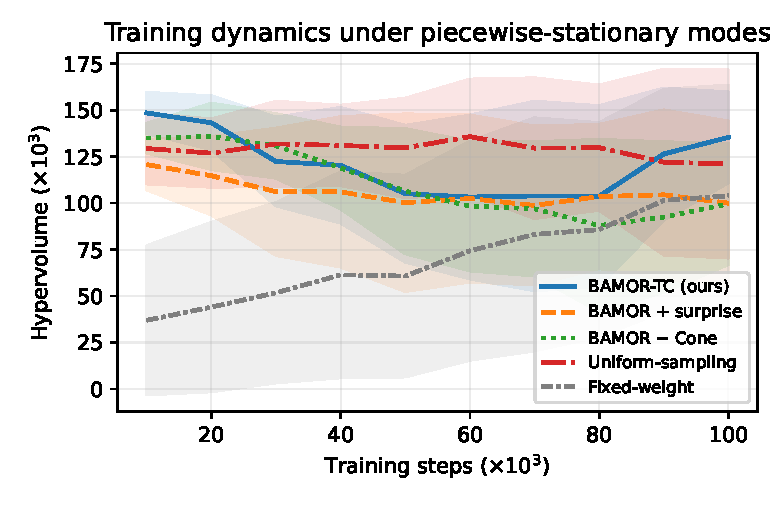
\includegraphics[width=0.72\linewidth]{fig_training_curves_v2.pdf}
\caption{Overall HV during training.  Shaded bands are $\pm1\sigma$ across 20 seeds.  BAMOR-TC (blue) starts high, loses ground in the middle training window, then recovers after $80$k steps and finishes with the highest mean and a tighter final band than Uniform.  Uniform (red) is steadier through the middle but ends lower.  BAMOR $+$ surprise (orange) and BAMOR $-$ Cone (green) finish well below BAMOR-TC.  Fixed-weight (grey) improves late but remains high-variance.}
\label{fig:training_curves}
\end{figure}

Fig.~\ref{fig:training_curves} shows HV trajectories during training.  Two qualitative patterns stand out.  First, BAMOR-TC is not a pointwise-dominant training curve: it starts high, falls below Uniform in the middle window, and then recovers sharply by the final evaluations.  The defensible claim is final HV and lower final variance, not monotone dominance at every checkpoint.  Second, both adaptive ablations have lower final sample means than BAMOR-TC. The paired synthetic comparison and ablation limitations above restrict a causal interpretation of these curves.

% ── 6.6 Continuous-control stress test ─────────────────────────────────────

\clearpage
\subsection{Historical Continuous-Control Comparison}
\label{app:historical_continuous}

The original 20-seed, 50k-step v23 study used 19 BAMOR actor snapshots but
one CAPQL actor. Its overall evaluator advanced a persistent mode schedule
across episodes, weights and actors. Changing the number or order of candidates
therefore changed evaluation conditions as well as the evaluated policy set.
Table~\ref{tab:mujoco_3d_policy_set} is retained as a historical record and is
not used in the matched-comparison conclusions.

\begin{table}[t]
\centering\footnotesize
\caption{Historical exploratory continuous-control results, retained with their original metric. HV is in billions (B). BAMOR-v23 and v22 use 19 actor snapshots; CAPQL uses its final actor. The overall evaluator advances a persistent mode schedule between candidates, so this is not an archive-matched or common-distribution comparison. Bottom20 is the mean of the lowest 20\% of seeds; wins and two-sided Wilcoxon $p$ values describe this historical metric only. HalfCheetah has two objectives; Ant and Hopper have three.}
\label{tab:mujoco_3d_policy_set}
\begin{tabular}{llrrrrcc}
\toprule
Env & Method & Mean & Median & Bottom20 & Min & Wins & $p$ \\
\midrule
\multirow{4}{*}{HalfCheetah}
& Uniform & 0.001 & 0.000 & 0.000 & 0.000 & 20/20 & $<10^{-4}$ \\
& CAPQL & 0.004 & 0.003 & 0.001 & 0.000 & 14/20 & 0.0328 \\
& BAMOR-v22 & 0.006 & 0.006 & 0.003 & 0.002 & 11/20 & 0.5706 \\
& \textbf{BAMOR-v23} & \textbf{0.006} & 0.005 & \textbf{0.004} & \textbf{0.003} & -- & -- \\
\midrule
\multirow{6}{*}{Ant}
& Uniform & 12.671 & 9.460 & 2.584 & 2.185 & 20/20 & $<10^{-4}$ \\
& CAPQL & 10.137 & 4.466 & 2.665 & 2.292 & 20/20 & $<10^{-4}$ \\
& BAMOR & 13.769 & 16.661 & 2.931 & 2.381 & 20/20 & $<10^{-4}$ \\
& v5 MoE-template & 12.312 & 11.405 & 2.487 & 2.266 & 20/20 & $<10^{-4}$ \\
& v6 shared-head MoE & 13.441 & 16.136 & 2.587 & 2.185 & 20/20 & $<10^{-4}$ \\
& \textbf{BAMOR-v23} & \textbf{40.899} & \textbf{40.495} & \textbf{36.918} & \textbf{34.123} & -- & -- \\
\midrule
\multirow{6}{*}{Hopper}
& Uniform & 1.500 & 1.618 & 0.026 & 0.017 & 18/20 & 0.0001 \\
& CAPQL & 4.335 & 2.835 & 1.325 & 0.487 & 14/20 & 0.0973 \\
& BAMOR & 2.287 & 1.610 & 0.024 & 0.016 & 16/20 & 0.0014 \\
& v5 MoE-template & 2.412 & 2.368 & 0.408 & 0.027 & 17/20 & 0.0002 \\
& v6 shared-head MoE & 2.406 & 2.347 & 0.459 & 0.018 & 20/20 & $<10^{-4}$ \\
& \textbf{BAMOR-v23} & \textbf{6.193} & \textbf{4.818} & \textbf{2.851} & \textbf{2.804} & -- & -- \\
\bottomrule
\end{tabular}
\end{table}


The historical locked-mode diagnostic used restricted preference grids and
unmatched episode resets. Mean mode-wise archive/final HV, v23 versus CAPQL,
was 3.032M/2.221M on HalfCheetah, 2.096B/1.838B on Ant and 3.357B/1.914B
on Hopper. Even there, HalfCheetah mode 3 favored CAPQL, 1.653M versus 0.827M.
The current main-text comparisons replace these settings with common locked
modes, full-simplex grids and episode reset seeds.
\FloatBarrier

\clearpage
\section{Preliminaries}
% ════════════════════════════════════════════════════════════════════════════

\subsection{Multi-objective piecewise-stationary MDP}

\begin{definition}[MO-PS-MDP]
\label{def:mopsmdp}
A \emph{Multi-Objective Piecewise-Stationary MDP} is a sequence of multi-objective MDPs $\{\mathcal{M}_k\}_{k=1}^\infty$ where each $\mathcal{M}_k = (\mathcal{S}, \mathcal{A}, P_k, \mathbf{R}_k, \gamma)$ shares state and action spaces but has distinct:
\begin{itemize}
    \item Transition kernels $P_k : \mathcal{S} \times \mathcal{A} \to \Delta(\mathcal{S})$;
    \item \emph{Vector-valued} reward functions $\mathbf{R}_k : \mathcal{S} \times \mathcal{A} \to \mathbb{R}^m$, where $m$ is the number of objectives;
    \item Discount factor $\gamma \in [0, 1)$ shared across all modes.
\end{itemize}
Regime switches occur at unknown times $t_1 < t_2 < \cdots$.  Between consecutive switches, the MDP is stationary.
\end{definition}

\subsection{Vector-valued Q-functions and metrics}

The Q-function is vector-valued: $\mathbf{Q} : \mathcal{S} \times \mathcal{A} \to \mathbb{R}^m$, where $Q_i(s,a)$ is the expected discounted return for objective $i$.  The function space is equipped with the product $L_\infty$ (sup-norm) metric:
\begin{equation}
    \mathrm{dist}(\mathbf{Q}_1, \mathbf{Q}_2) = \sup_{(s,a) \in \mathcal{S} \times \mathcal{A}} \sup_{i \in \{1,\ldots,m\}} |Q_{1,i}(s,a) - Q_{2,i}(s,a)|.
    \label{eq:dist}
\end{equation}
In Lean~4, this is realized as the nested Pi metric: $\mathcal{S} \times \mathcal{A} \to \mathrm{Fin}\, m \to \mathbb{R}$, where each layer inherits the \texttt{PseudoMetricSpace} instance from Mathlib.

\subsection{Preference-weighted scalarization}

Given a preference weight $w \in \Delta^{m-1}$ (the probability simplex: $w_i \ge 0$, $\sum_i w_i = 1$), the scalarized Q-value is:
\begin{equation}
    Q_w(s,a) = \langle w, \mathbf{Q}(s,a) \rangle = \sum_{i=1}^m w_i \cdot Q_i(s,a).
    \label{eq:scalarize}
\end{equation}
The scalarized greedy value is $V_w(s) = \max_a Q_w(s,a)$. For a fixed vector $\mathbf Q(s,a)$, consider the auxiliary function
\begin{equation}
    f_\eta(w; s,a) = \langle w, \mathbf{Q}(s,a) \rangle - \eta \|w\|^2,
    \label{eq:regularized_scalarize}
\end{equation}
where $\eta>0$ makes this function strictly concave in $w$. This does not imply a bijection between preferences and achievable Pareto returns. If $w$ is a sampled input independent of actor parameters, the quadratic term has zero actor gradient.

\subsection{BAPR: Bayesian Amnesic Piecewise-Robust RL}

BAMOR builds upon the BAPR framework~\cite{Zhang2025BAPR}, which integrates Bayesian Online Change Detection (BOCD)~\cite{Adams2007BOCD} with robust ensemble SAC~\cite{Haarnoja2018SAC, Zhang2025RESAC}.  Key properties we import:
\begin{itemize}
    \item \textbf{BAPR operator:} $\mathcal{T}^{\mathrm{BAPR}}_\rho Q = \sum_h \rho(h) \mathcal{T}_h Q$ is a $\gamma$-contraction when $\rho$ is frozen.
    \item \textbf{Bayesian belief update:} $\rho'(h) = \rho(h) L(h) / Z$ preserves $\rho' \ge 0$ and $\sum_h \rho'(h) = 1$.
    \item \textbf{Counterexample:} Q-dependent beliefs break contraction when $\gamma + \lambda\Delta \ge 1$.
\end{itemize}

\begin{remark}[What changes from BAPR to BAMOR]
\label{rem:bapr_to_bamor}
The extension from BAPR (scalar $Q : \mathcal{S} \times \mathcal{A} \to \mathbb{R}$) to BAMOR (vector $\mathbf{Q} : \mathcal{S} \times \mathcal{A} \to \mathbb{R}^m$) is not a trivial generalization.  It introduces:
\begin{enumerate}
    \item \textbf{Nested metric:} The $L_\infty$ metric on $\mathbb{R}^m$-valued functions requires two layers of Pi-metric unpacking in the contraction proof.
    \item \textbf{Scalarization layer:} An entirely new non-expansiveness proof for the weighted sum, and its composition with component-wise contraction.
    \item \textbf{Weight space geometry:} Lipschitz continuity in $w$, strong concavity, and the anchor-shift theory have no analogue in single-objective BAPR.
    \item \textbf{Component-wise drift:} The Target Cone theory exploits the vector structure of the drift, which collapses to a scalar in BAPR.
\end{enumerate}
\end{remark}


% ════════════════════════════════════════════════════════════════════════════
\section{The BAMOR Framework}
\label{sec:framework}
% ════════════════════════════════════════════════════════════════════════════

\subsection{Mode-conditional multi-objective Bellman operator}

For each environment mode $h \in \mathcal{H}$ (finite, non-empty), we define the mode-conditional multi-objective operator acting on vector-valued Q-functions.

\begin{definition}[Mode-conditional operator --- Lean: \texttt{T\_mode\_mo}]
\label{def:t_mode_mo}
\begin{equation}
    [\mathcal{T}_h \mathbf{Q}](s,a,i) = R_h(s,a,i) + \gamma \left( \sum_{s' \in \mathcal{S}} P_h(s'|s,a) \underbrace{\max_{a' \in \mathcal{A}} Q_i(s',a')}_{V_i^{\mathbf{Q}}(s')} - \lambda_{\mathrm{epi}} \Gamma_{\mathrm{epi},h}(s,a,i) - \kappa_i \right),
    \label{eq:mode_operator}
\end{equation}
where:
\begin{itemize}
    \item $R_h(s,a,i)$ is the reward for objective $i$ under mode $h$;
    \item $V_i^{\mathbf{Q}}(s') = \max_{a'} Q_i(s',a')$ is the per-component value function;
    \item $\Gamma_{\mathrm{epi},h}(s,a,i)$ is the per-objective epistemic penalty from the frozen target ensemble;
    \item $\kappa_i$ is the per-objective aleatoric penalty from frozen critic weights (cf.\ RE-SAC~\cite{Zhang2025RESAC}).
\end{itemize}
\end{definition}

\begin{remark}[Per-objective penalties]
Unlike BAPR (scalar $\kappa$, scalar $\Gamma_{\mathrm{epi}}$), BAMOR uses \emph{per-objective} penalties $\kappa_i$ and $\Gamma_{\mathrm{epi},h}(s,a,i)$.  This allows different objectives to have different aleatoric noise levels and epistemic uncertainty---critical for multi-objective settings where, e.g., speed measurement is noisy but headway measurement is precise.
\end{remark}

\subsection{BAMOR operator: belief-weighted multi-objective mixture}

\begin{definition}[BAMOR operator --- Lean: \texttt{T\_BAMOR}]
\label{def:t_bamor}
The BAMOR operator is the belief-weighted mixture over modes:
\begin{equation}
    [\mathcal{T}^{\mathrm{BAMOR}}_\rho \mathbf{Q}](s,a,i) = \sum_{h \in \mathcal{H}} \rho(h) \cdot [\mathcal{T}_h \mathbf{Q}](s,a,i),
    \label{eq:bamor_operator}
\end{equation}
where $\rho : \mathcal{H} \to [0,1]$ is a belief distribution satisfying $\rho(h) \ge 0$ for all $h$ and $\sum_h \rho(h) = 1$, \textbf{frozen during each Bellman backup}.
\end{definition}

\begin{remark}[Frozen beliefs: necessary, not convenient]
As proven in the BAPR counterexample~\cite{Zhang2025BAPR}, Q-dependent beliefs break contraction.  The frozen-belief design is an essential structural requirement, not a simplification.  The belief is updated \emph{between} backup iterations using the Mahalanobis surprise signal.
\end{remark}

\subsection{Belief-update rules: a separable design choice}
\label{sec:belief_rules}

The contraction proof (\S\ref{sec:contraction}) holds for \emph{any} belief $\rho$ that is frozen across a single backup iteration.  The practical question is how to produce $\rho$ at deployment.  We consider three regimes, in increasing order of algorithmic commitment:

\textbf{(B1) Oracle / mode-labelled belief.}  When the deployment pipeline exposes a mode label $h^\star$ (e.g., a weather code, a traffic-light phase, or a diurnal indicator), set $\rho = \delta_{h^\star}$.  Contraction holds trivially; the cone estimator receives clean per-mode data.

\textbf{(B2) Static uniform belief ($\rho_h = 1/|\mathcal{H}|$).}  When no label is available and we are unwilling to trust an online estimator, freeze the belief at the uniform prior.  The cone estimator then accumulates a \emph{global} anchor that averages over the modes visited during training---a coarse simplification, but one that gives the best empirical results in our high-noise 2-D benchmark (\S\ref{sec:exp_ablation}, variant \texttt{BAMOR-TC}).  Intuitively, the cone-only concentration still filters out low-yield corners of the simplex under the active substrate, which is where most of the wasted exploration under uniform-$w$ sampling occurs.

\textbf{(B3) Online Mahalanobis change-point belief.}  A fully automatic belief update that turns reward residuals into a Mahalanobis $\chi^2$ surprise and triggers a round-robin mode reassignment on threshold crossings:
\begin{align}
    d^2_{\mathrm{Mah}}(\boldsymbol{\xi}, \mathrm{prec}) &= \sum_{i=1}^m \mathrm{prec}_i \cdot \xi_i^2, \qquad
    L(h) = \exp\bigl(-\tfrac{1}{2} d^2_{\mathrm{Mah}}(\boldsymbol{\xi}(h), \mathrm{prec})\bigr).
    \label{eq:mahalanobis}
\end{align}
The Mahalanobis likelihood is strictly positive, so the normalisation $Z = \sum_h \rho(h) L(h) > 0$ automatically (Lean: \texttt{mahalanobis\_normalization\_pos})---this eliminates the ad-hoc $Z > 0$ hypothesis required in generic BAPR.

\textbf{A caveat from our experiments.}  Variant (B3) is elegant in theory and is the mechanism we originally designed.  However, in our current 20-seed 2-objective synthetic benchmark it is not the empirically safest default: enabling the online Mahalanobis detector lowers overall HV from $136.2{\times}10^3$ to $96.9{\times}10^3$ and increases the seed-level std from $23.6{\times}10^3$ to $43.8{\times}10^3$.  The detector also leaves one severe Mode-1 collapse seed ($\mathrm{HV}_{\mathrm{Mode\,1}}<10^3$).  We therefore \emph{do not advocate (B3) as the default recipe}; our reported ``BAMOR'' is variant (B2), and (B3) is evaluated as a secondary ablation to quantify the performance loss caused by a miscalibrated automatic rule.  Designing a well-calibrated online belief update for settings where mode labels are unavailable is an open problem we discuss in \S\ref{sec:limits}.

\subsection{Substrate constraints and Target Cone}
\label{sec:target_cone}

\begin{figure}[t]
\centering
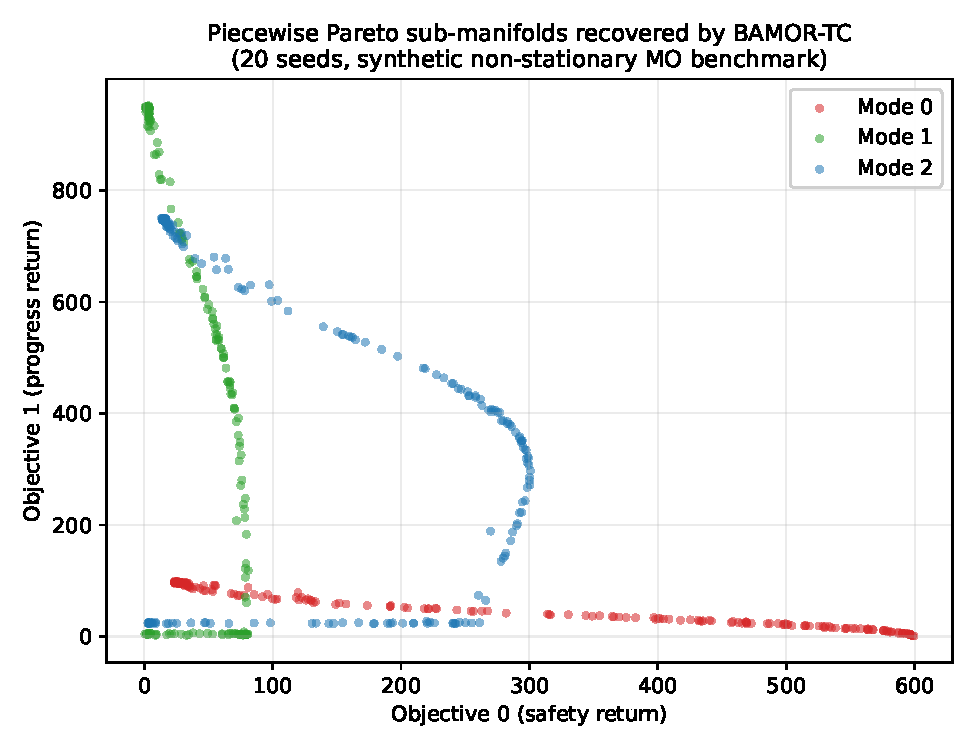
\includegraphics[width=0.78\linewidth]{fig_submfld_hero.pdf}
\caption{The piecewise Pareto sub-manifold structure that BAMOR-TC is designed to exploit, here recovered empirically from $20$ seeds on the synthetic non-stationary MO benchmark.  Each mode's achievable trade-off is a mostly separated, low-dimensional arc: Mode~0 (red) is near-horizontal because progress is strongly capped; Mode~1 (green) is near-vertical because safety is strongly capped; Mode~2 (blue) admits a broader elbow.  The global-smooth-front view is therefore not the right description for this benchmark.  BAMOR's \emph{Target Cone} restricts the weight sampler to the relevant arc per mode (\S\ref{sec:framework}).}
\label{fig:submfld_hero}
\end{figure}

\begin{definition}[Substrate Constraint]
\label{def:substrate}
An environment mode $h$ imposes a \emph{substrate constraint} on objective $i$ if the physical dynamics under mode $h$ bound the achievable improvement in objective $i$ regardless of the policy:
\begin{equation}
    \max_\pi V_i^\pi(s) \le B_{h,i} \quad \text{for all } s \in \mathcal{S},
\end{equation}
where $B_{h,i}$ is a mode-dependent physical ceiling that may be much lower than the ceiling under other modes.  Fig.~\ref{fig:submfld_hero} shows what this looks like in practice: each mode's achievable returns lie on a different arc.
\end{definition}

\begin{definition}[Target Cone --- Lean: \texttt{ModeConeConstraint}]
\label{def:target_cone}
For each mode $h$, the \emph{Target Cone} $\mathcal{C}_h \subset \Delta^{m-1}$ is characterized by:
\begin{itemize}
    \item A \emph{preference anchor} $w_{\mathrm{anchor}}(h) \in \Delta^{m-1}$: the physical center of the cone, satisfying $w_{\mathrm{anchor}}(h,i) \ge 0$ and $\sum_i w_{\mathrm{anchor}}(h,i) = 1$;
    \item A \emph{cone radius} $r_h > 0$: $\mathcal{C}_h = \{w \in \Delta^{m-1} : \|w - w_{\mathrm{anchor}}(h)\|_2 \le r_h\}$.
\end{itemize}
Weights outside $\mathcal{C}_h$ remain valid preferences. The cone is a chosen training-allocation region, not a characterization of all achievable returns.
\end{definition}

\begin{example}[Target Cones for bus transit]
\label{ex:cones}
For an illustrative two-objective setting with $m=2$:
\begin{center}
\begin{tabular}{lccc}
\toprule
\textbf{Mode} & $w_{\mathrm{anchor}}$ & \textbf{Cone interval} & \textbf{Physical reason} \\
\midrule
Normal & $(0.5, 0.5)$ & $w_{\mathrm{headway}} \in [0.3, 0.7]$ & Free trade-off \\
Severe congestion & $(0.95, 0.05)$ & $w_{\mathrm{headway}} \in [0.85, 1.0]$ & Speed ceiling hit \\
Demand surge & $(0.2, 0.8)$ & $w_{\mathrm{headway}} \in [0.1, 0.4]$ & Must move passengers \\
\bottomrule
\end{tabular}
\end{center}
\end{example}

\begin{definition}[Belief-weighted anchor --- Lean: \texttt{belief\_weighted\_anchor}]
\label{def:belief_anchor}
The belief-weighted anchor aggregates mode-specific anchors:
\begin{equation}
    \tilde{w}_i = \sum_{h \in \mathcal{H}} \rho(h) \cdot w_{\mathrm{anchor}}(h, i).
    \label{eq:belief_anchor}
\end{equation}
When $\rho$ concentrates on mode $h_0$ (after surprise detection), $\tilde{w} \approx w_{\mathrm{anchor}}(h_0)$.  During uncertainty (diffuse $\rho$), it smoothly interpolates.
\end{definition}

\subsection{Anchor-shifted regularization}
\label{sec:anchor_reg}

For the auxiliary scalarization analysis, shift the quadratic center to a fixed anchor:
\begin{equation}
    f_{\mathrm{anchor}}(w; s,a) = \langle w, \mathbf{Q}(s,a) \rangle - \eta \|w - \tilde{w}\|^2.
    \label{eq:anchor_reg}
\end{equation}
The curvature with respect to $w$ is unchanged (Theorem~\ref{thm:anchor_concavity}). In the implemented actor update, $w$ and the anchor are fixed inputs, so this term has no actor gradient and is omitted.

\subsection{Context-aware weight sampling}
\label{sec:sampling}

The current BAMOR-TC sampler concentrates a Dirichlet distribution around the estimated anchor:
\begin{equation}
    w\sim\mathrm{Dirichlet}(\alpha),\qquad
    \alpha_i=\kappa_{\mathrm{eff}}\tilde w_i+10^{-3},
\end{equation}
where the effective concentration is scaled by the estimated cone radius. This distribution has full simplex-interior support; it is not uniform sampling from, or hard truncation to, $\mathcal C_h$. A radius therefore specifies concentration, not a guaranteed support boundary. BAMOR-v23 instead uses the selected arm's uniform, stratified, mixed or extreme-preference sampler.

\section{Theoretical Analysis}
\label{sec:theory}
% ════════════════════════════════════════════════════════════════════════════

All theorems in this section are machine-verified in Lean~4/Mathlib with no \texttt{sorry}.  Full proof details with complete derivations are in Appendix~\ref{app:contraction}--\ref{app:improvement}.  We state each result with proof sketches that highlight the key mathematical moves.

\subsection{BAMOR is a gamma-contraction (Parts I--VI)}
\label{sec:contraction}

The proof proceeds bottom-up: per-component max properties $\to$ per-mode properties $\to$ mixture properties $\to$ Banach fixed point.

\subsubsection{Component-wise max properties}

\begin{lemma}[Component-wise max is 1-Lipschitz --- Lean: \texttt{max\_over\_a\_comp\_nonexpansive}]
\label{lem:max_lip}
If $|Q_{1,i}(s,a) - Q_{2,i}(s,a)| \le \varepsilon$ for all $s,a,i$, then $|V_i^{\mathbf{Q}_1}(s) - V_i^{\mathbf{Q}_2}(s)| \le \varepsilon$ for all $s,i$.
\end{lemma}

\begin{proof}
For the upper bound: for any action $a$, $Q_{1,i}(s,a) \le Q_{2,i}(s,a) + \varepsilon \le V_i^{\mathbf{Q}_2}(s) + \varepsilon$.  Taking $\max_a$ gives $V_i^{\mathbf{Q}_1}(s) \le V_i^{\mathbf{Q}_2}(s) + \varepsilon$.  Symmetrically for the lower bound.  The Lean proof proceeds via \texttt{Finset.sup'\_le} applied to the finite action space.
\end{proof}

\subsubsection{Per-mode contraction}

\begin{lemma}[Per-mode pointwise bound --- Lean: \texttt{t\_mode\_mo\_pointwise\_bound}]
\label{lem:mode_bound}
If $\mathrm{dist}(\mathbf{Q}_1, \mathbf{Q}_2) \le \varepsilon$, then $|[\mathcal{T}_h \mathbf{Q}_1](s,a,i) - [\mathcal{T}_h \mathbf{Q}_2](s,a,i)| \le \gamma\varepsilon$ for all $h,s,a,i$.
\end{lemma}

\begin{proof}
The frozen penalties ($R_h$, $\Gamma_{\mathrm{epi},h}$, $\kappa_i$) cancel in the difference.  By Lemma~\ref{lem:max_lip}: $|V_i^{\mathbf{Q}_1}(s') - V_i^{\mathbf{Q}_2}(s')| \le \varepsilon$.  Then:
\begin{align}
    |[\mathcal{T}_h \mathbf{Q}_1 - \mathcal{T}_h \mathbf{Q}_2](s,a,i)| &= \gamma \left|\sum_{s'} P_h(s'|s,a)(V_i^{\mathbf{Q}_1}(s') - V_i^{\mathbf{Q}_2}(s'))\right| \notag \\
    &\le \gamma \sum_{s'} P_h(s'|s,a) |V_i^{\mathbf{Q}_1}(s') - V_i^{\mathbf{Q}_2}(s')| \quad \text{(triangle, $P_h \ge 0$)} \notag \\
    &\le \gamma \sum_{s'} P_h(s'|s,a) \cdot \varepsilon = \gamma\varepsilon \cdot \underbrace{\sum_{s'} P_h(s'|s,a)}_{=1}. \qedhere
\end{align}
\end{proof}

\subsubsection{Main contraction theorem}

\begin{theorem}[BAMOR gamma-contraction --- Lean: \texttt{bamor\_contraction}]
\label{thm:bamor_contraction}
Under (A0)--(A4), the BAMOR operator satisfies:
\begin{equation}
    \mathrm{dist}(\mathcal{T}^{\mathrm{BAMOR}}_\rho \mathbf{Q}_1, \mathcal{T}^{\mathrm{BAMOR}}_\rho \mathbf{Q}_2) \le \gamma \cdot \mathrm{dist}(\mathbf{Q}_1, \mathbf{Q}_2).
\end{equation}
\end{theorem}

\begin{proof}
Let $\varepsilon = \mathrm{dist}(\mathbf{Q}_1, \mathbf{Q}_2)$.  We need to show $\mathrm{dist}(\mathcal{T}\mathbf{Q}_1, \mathcal{T}\mathbf{Q}_2) \le \gamma\varepsilon$.  By Eq.~\eqref{eq:dist}, this requires showing $|[\mathcal{T}\mathbf{Q}_1](s,a,i) - [\mathcal{T}\mathbf{Q}_2](s,a,i)| \le \gamma\varepsilon$ for all $(s,a,i)$.

Expanding the BAMOR operator:
\begin{align}
    &|[\mathcal{T}^{\mathrm{BAMOR}}_\rho \mathbf{Q}_1](s,a,i) - [\mathcal{T}^{\mathrm{BAMOR}}_\rho \mathbf{Q}_2](s,a,i)| \notag \\
    &= \left|\sum_{h} \rho(h) \left([\mathcal{T}_h \mathbf{Q}_1](s,a,i) - [\mathcal{T}_h \mathbf{Q}_2](s,a,i)\right)\right| \notag \\
    &\le \sum_{h} \rho(h) \left|[\mathcal{T}_h \mathbf{Q}_1](s,a,i) - [\mathcal{T}_h \mathbf{Q}_2](s,a,i)\right| \quad \text{(triangle inequality, $\rho(h) \ge 0$ by (A3))} \notag \\
    &\le \sum_{h} \rho(h) \cdot \gamma\varepsilon \quad \text{(per-mode bound, Lemma~\ref{lem:mode_bound})} \notag \\
    &= \gamma\varepsilon \cdot \sum_{h} \rho(h) = \gamma\varepsilon. \quad \text{($\sum \rho = 1$ by (A4))}
\end{align}

The Lean proof (function \texttt{bamor\_dist\_le}) proceeds by:
\begin{enumerate}
    \item Setting $\varepsilon := \mathrm{dist}(\mathbf{Q}_1, \mathbf{Q}_2)$ and showing $0 \le \varepsilon$;
    \item Applying \texttt{dist\_pi\_le\_iff} twice to unpack the nested Pi metric, reducing to pointwise bounds;
    \item Extracting pointwise bounds $|Q_{1,i}(s,a) - Q_{2,i}(s,a)| \le \varepsilon$ from the dist assumption;
    \item Applying the mode-bound lemma and the triangle-inequality/normalization argument;
    \item Taking the supremum over $(s,a,i)$ via \texttt{dist\_pi\_le\_iff} in the reverse direction.
\end{enumerate}
The existential form $\exists k < 1, \forall \mathbf{Q}_1\,\mathbf{Q}_2,\, \mathrm{dist}(\mathcal{T}\mathbf{Q}_1, \mathcal{T}\mathbf{Q}_2) \le k \cdot \mathrm{dist}(\mathbf{Q}_1, \mathbf{Q}_2)$ follows by witnessing $k := \gamma$ and $\gamma < 1$.
\end{proof}

\subsubsection{Blackwell conditions (Lean: Parts I)}

For completeness and to bridge to the classical theory, we also verify both Blackwell conditions:

\begin{lemma}[BAMOR monotonicity --- Blackwell (i) --- Lean: \texttt{bamor\_monotonicity}]
If $\mathbf{Q}_1 \le \mathbf{Q}_2$ pointwise, then $\mathcal{T}^{\mathrm{BAMOR}}_\rho \mathbf{Q}_1 \le \mathcal{T}^{\mathrm{BAMOR}}_\rho \mathbf{Q}_2$ pointwise.
\end{lemma}

\begin{lemma}[BAMOR discounting --- Blackwell (ii) --- Lean: \texttt{bamor\_discounting}]
For any constant vector $\mathbf{c} \in \mathbb{R}^m$: $\mathcal{T}^{\mathrm{BAMOR}}_\rho(\mathbf{Q} + \mathbf{c}) = \mathcal{T}^{\mathrm{BAMOR}}_\rho \mathbf{Q} + \gamma \mathbf{c}$.
\end{lemma}

\begin{proof}
The discounting proof is where $\sum_h \rho(h) = 1$ (A4) is essential.  Per-mode: $\mathcal{T}_h(\mathbf{Q} + \mathbf{c})(s,a,i) = \mathcal{T}_h\mathbf{Q}(s,a,i) + \gamma c_i$ (because $\max_a (Q_i(s,a) + c_i) = \max_a Q_i(s,a) + c_i$ and $\sum_{s'} P_h = 1$).  Mixing: $\sum_h \rho(h)(\mathcal{T}_h\mathbf{Q}(s,a,i) + \gamma c_i) = \mathcal{T}^{\mathrm{BAMOR}}\mathbf{Q}(s,a,i) + \gamma c_i \cdot \sum_h \rho(h) = \mathcal{T}^{\mathrm{BAMOR}}\mathbf{Q}(s,a,i) + \gamma c_i$.
\end{proof}

\subsubsection{Banach fixed point (Part VI)}

\begin{corollary}[Existence and uniqueness]
\label{cor:fixed_point}
$\mathcal{T}^{\mathrm{BAMOR}}_\rho$ has a unique fixed point $\mathbf Q^*$ in the finite-dimensional vector-value space. The independent coordinate maximizations do not imply joint achievability by one policy.

For example, with one state, zero penalties, and actions with rewards $(1,0)$ and $(0,1)$, the componentwise optimal state value is $(1/(1-\gamma),1/(1-\gamma))$. Every realizable policy has the sum of its two state-value coordinates equal to $1/(1-\gamma)$. Thus the componentwise fixed-point construction must not be identified with an achievable Pareto-optimal policy.
\end{corollary}

\begin{proof}
\textbf{Uniqueness:} If $\mathcal{T}\mathbf{Q}_1 = \mathbf{Q}_1$ and $\mathcal{T}\mathbf{Q}_2 = \mathbf{Q}_2$, then $\mathrm{dist}(\mathbf{Q}_1, \mathbf{Q}_2) = \mathrm{dist}(\mathcal{T}\mathbf{Q}_1, \mathcal{T}\mathbf{Q}_2) \le \gamma \mathrm{dist}(\mathbf{Q}_1, \mathbf{Q}_2)$.  Since $\gamma < 1$ and $\mathrm{dist} \ge 0$: $(1 - \gamma)\mathrm{dist} \le 0$, forcing $\mathrm{dist} = 0$.

\textbf{Existence:} The Lean proof bridges to Mathlib's \texttt{ContractingWith.exists\_fixedPoint}, starting from $\mathbf{Q}_0 = 0$.  The key steps: (i)~\texttt{bamor\_lipschitzWith} shows Lipschitz constant $\gamma$; (ii)~\texttt{bamor\_contractingWith} packages this with $\gamma < 1$; (iii)~the finite type ensures \texttt{edist} from $\mathbf{Q}_0$ to $\mathcal{T}\mathbf{Q}_0$ is finite.
\end{proof}

\subsubsection{Contraction after belief update (Parts II, IV)}

\begin{corollary}[Post-update contraction --- Lean: \texttt{bamor\_contraction\_after\_update}]
If $\rho$ is updated to $\rho'$ via Bayesian update with $Z > 0$, then $\mathcal{T}^{\mathrm{BAMOR}}_{\rho'}$ is a $\gamma$-contraction.
\end{corollary}

\begin{corollary}[Mahalanobis contraction --- Lean: \texttt{bamor\_contraction\_mahalanobis}]
\label{cor:mahalanobis}
With Mahalanobis likelihood, the $Z > 0$ requirement is automatically satisfied from prior support ($\exists h, \rho(h) > 0$), providing a stronger guarantee than generic BAPR.
\end{corollary}


\subsection{Scalarized contraction and weight sensitivity (Parts VII--VIII)}
\label{sec:scalarized}

\begin{theorem}[Scalarized BAMOR contraction --- Lean: \texttt{scalarized\_bamor\_contraction}]
\label{thm:scalarized_contraction}
For any $w \in \Delta^{m-1}$ and any $(s,a)$:
\begin{equation}
    |\langle w, \mathcal{T}^{\mathrm{BAMOR}}_\rho \mathbf{Q}_1(s,a) \rangle - \langle w, \mathcal{T}^{\mathrm{BAMOR}}_\rho \mathbf{Q}_2(s,a) \rangle| \le \gamma \cdot \mathrm{dist}(\mathbf{Q}_1, \mathbf{Q}_2).
\end{equation}
\end{theorem}

\begin{proof}
This composes two results:
\begin{enumerate}
    \item \textbf{Part I (contraction):} $|[\mathcal{T}\mathbf{Q}_1](s,a,i) - [\mathcal{T}\mathbf{Q}_2](s,a,i)| \le \gamma\varepsilon$ for all $i$;
    \item \textbf{Part III (non-expansiveness):} $|\sum_i w_i (f_i - g_i)| \le \sum_i w_i |f_i - g_i| \le \max_i |f_i - g_i|$ when $w \ge 0, \sum w_i = 1$.
\end{enumerate}
Combining: $|\langle w, \mathcal{T}\mathbf{Q}_1(s,a) - \mathcal{T}\mathbf{Q}_2(s,a) \rangle| \le \gamma\varepsilon$.
\end{proof}

\begin{remark}[Why this matters]
Theorem~\ref{thm:scalarized_contraction} bounds the scalarized output difference by $\gamma$ times the vector sup-norm input difference. It is not a contraction statement in the scalarized-input pseudometric, nor a convergence result for preference-conditioned neural control.
\end{remark}

\begin{lemma}[Weight Lipschitz --- Lean: \texttt{scalarize\_lipschitz\_in\_w}]
\label{lem:weight_lipschitz}
For Q-values bounded by $B$ ($|Q_i(s,a)| \le B$ for all $s,a,i$):
\begin{equation}
    |\langle w_1, \mathbf{Q}(s,a) \rangle - \langle w_2, \mathbf{Q}(s,a) \rangle| \le B \cdot \|w_1 - w_2\|_1.
\end{equation}
\end{lemma}

\begin{proof}
$|\sum_i (w_{1,i} - w_{2,i}) Q_i(s,a)| \le \sum_i |w_{1,i} - w_{2,i}| \cdot |Q_i(s,a)| \le B \sum_i |w_{1,i} - w_{2,i}|$.
\end{proof}

\begin{corollary}[Pareto value Lipschitz --- Lean: \texttt{pareto\_val\_lipschitz\_in\_w}]
$|V_{w_1}(s) - V_{w_2}(s)| \le B \cdot \|w_1 - w_2\|_1$.
\end{corollary}

This result quantifies the ``nearby preferences $\Rightarrow$ nearby values'' property, justifying the cone-restricted sampling: if the sampled $w$ is within radius $r_h$ of the anchor, the resulting value differs by at most $B \cdot 2r_h$ from the anchor's value.


\subsection{Strong concavity and anchor-shifted regularization (Parts IX, XI, XIII)}
\label{sec:anchor}

\subsubsection{Auxiliary quadratic scalarization (Part IX)}

\begin{theorem}[Strong concavity --- Lean: \texttt{regularized\_scalarize\_strongly\_concave}]
\label{thm:strong_concavity}
For any $\eta, t \in \mathbb{R}$ and any $w_1, w_2$:
\begin{equation}
    f_\eta(tw_1 + (1{-}t)w_2) \ge t \cdot f_\eta(w_1) + (1{-}t) \cdot f_\eta(w_2) + \eta t(1{-}t)\|w_1 - w_2\|^2,
\end{equation}
where $f_\eta(w) = \langle w, \mathbf{Q}(s,a) \rangle - \eta\|w\|^2$.
\end{theorem}

\begin{proof}
The proof uses two ingredients:
\begin{enumerate}
    \item \textbf{Linearity of scalarization:} $\langle tw_1 + (1{-}t)w_2, \mathbf{Q} \rangle = t\langle w_1, \mathbf{Q} \rangle + (1{-}t)\langle w_2, \mathbf{Q} \rangle$ (Lean: \texttt{scalarize\_affine\_in\_w}).
    \item \textbf{Parallelogram identity:} $\|tw_1 + (1{-}t)w_2\|^2 + t(1{-}t)\|w_1 - w_2\|^2 = t\|w_1\|^2 + (1{-}t)\|w_2\|^2$ (Lean: \texttt{weight\_norm\_sq\_convex\_identity}).
\end{enumerate}
Substituting (1) and rearranging (2) into the definition of $f_\eta$:
\begin{align}
    f_\eta(tw_1 + (1{-}t)w_2) &= t\langle w_1, \mathbf{Q} \rangle + (1{-}t)\langle w_2, \mathbf{Q} \rangle - \eta\|tw_1 + (1{-}t)w_2\|^2 \\
    &= t\langle w_1, \mathbf{Q} \rangle + (1{-}t)\langle w_2, \mathbf{Q} \rangle - \eta(t\|w_1\|^2 + (1{-}t)\|w_2\|^2 - t(1{-}t)\|w_1 - w_2\|^2) \\
    &= tf_\eta(w_1) + (1{-}t)f_\eta(w_2) + \eta t(1{-}t)\|w_1 - w_2\|^2.
\end{align}
The gap $\eta t(1{-}t)\|w_1 - w_2\|^2 > 0$ when $\eta > 0$, $t \in (0,1)$, $w_1 \ne w_2$, guaranteeing strict concavity.
\end{proof}

\subsubsection{Anchor-shifted regularization (Part XI)}

\begin{theorem}[Anchor-shifted strong concavity]
\label{thm:anchor_concavity}
\emph{Lean: \texttt{anchor\_regularized\_strongly\_concave}.}

Shifting the regularization center to any $w_{\mathrm{anchor}}$ preserves the \textbf{identical} strong concavity gap:
\begin{equation}
    f_{\mathrm{anchor}}(tw_1 + (1{-}t)w_2) \ge tf_{\mathrm{anchor}}(w_1) + (1{-}t)f_{\mathrm{anchor}}(w_2) + \eta t(1{-}t)\|w_1 - w_2\|^2,
\end{equation}
where $f_{\mathrm{anchor}}(w) = \langle w, \mathbf{Q}(s,a) \rangle - \eta\|w - w_{\mathrm{anchor}}\|^2$.
\end{theorem}

\begin{proof}
The key insight is a change of variables: let $u = w - w_{\mathrm{anchor}}$.
\begin{enumerate}
    \item The convex combination shifts: $t w_1 + (1{-}t)w_2 - w_{\mathrm{anchor}} = t(w_1 - w_{\mathrm{anchor}}) + (1{-}t)(w_2 - w_{\mathrm{anchor}}) = tu_1 + (1{-}t)u_2$.
    \item Apply the parallelogram identity to $u_1, u_2$: $$\|tu_1 + (1{-}t)u_2\|^2 = t\|u_1\|^2 + (1{-}t)\|u_2\|^2 - t(1{-}t)\|u_1 - u_2\|^2.$$
    \item The anchor cancels in the difference: $u_1 - u_2 = (w_1 - w_{\mathrm{anchor}}) - (w_2 - w_{\mathrm{anchor}}) = w_1 - w_2$.
\end{enumerate}
Therefore $\|u_1 - u_2\|^2 = \|w_1 - w_2\|^2$, and the gap is \emph{identical} to the origin-centered case.  Geometrically: the Hessian $\nabla^2_w f_{\mathrm{anchor}} = -2\eta I$ is constant (translation-invariant).
\end{proof}

\begin{remark}[Physical significance]
This theorem concerns the curvature of an auxiliary function of $w$. It neither supplies an actor gradient for a sampled fixed weight nor establishes coverage of the Pareto front.
\end{remark}

\subsubsection{Mode Cone formalization and belief-anchor validity (Part XIII)}

\begin{theorem}[Belief-anchor is a valid preference --- Lean: \texttt{belief\_anchor\_valid\_preference}]
\label{thm:belief_anchor}
If each mode's anchor lies on $\Delta^{m-1}$ and $\rho$ is a valid belief, then the belief-weighted anchor $\tilde{w}$ (Eq.~\ref{eq:belief_anchor}) satisfies $\tilde{w}_i \ge 0$ for all $i$ and $\sum_i \tilde{w}_i = 1$.
\end{theorem}

\begin{proof}
Non-negativity: $\tilde{w}_i = \sum_h \rho(h) w_{\mathrm{anchor}}(h,i) \ge 0$ since each term is a product of non-negatives.  Normalization:
\begin{align}
    \sum_i \tilde{w}_i &= \sum_i \sum_h \rho(h) w_{\mathrm{anchor}}(h,i) = \sum_h \rho(h) \underbrace{\sum_i w_{\mathrm{anchor}}(h,i)}_{=1} = \sum_h \rho(h) = 1. \qedhere
\end{align}
\end{proof}

\begin{theorem}[Pipeline preserves strong concavity]
The anchor-shifted strong concavity (Theorem~\ref{thm:anchor_concavity}) holds when $w_{\mathrm{anchor}} = \tilde{w}$, proving that the entire BAMOR pipeline---surprise detection $\to$ belief update $\to$ anchor computation $\to$ regularized scalarization---preserves strong concavity at every step, for any valid belief $\rho$.
\end{theorem}


\subsection{Localized scalarized tracking bounds (Parts X, XII--XV)}
\label{sec:tracking}

This section formalizes when localized preference or operator choices improve a non-stationary tracking bound.  The comparison is conditional: the localized scalarized drift must be no larger than the global worst-component drift.  The result explains Target-Cone sampling and also applies to other selected operators that induce aligned non-negative preference weights.

\subsubsection{Global tracking under non-stationarity (Part X)}

\begin{theorem}[BAMOR robust tracking --- Lean: \texttt{bamor\_robust\_tracking}]
\label{thm:robust_tracking}
Given a sequence of $\gamma$-contractions $\{T_n\}$ (each from BAMOR with a different belief $\rho_n$) and bounded per-step target drift $\Delta$:
\begin{equation}
    \mathrm{dist}(\mathbf{Q}_n, \mathbf{Q}^*_n) \le \gamma^n \cdot D_0 + \frac{\Delta}{1 - \gamma},
    \label{eq:global_tracking}
\end{equation}
where $D_0 = \mathrm{dist}(\mathbf{Q}_0, \mathbf{Q}^*_0)$.
\end{theorem}

\begin{proof}
\textbf{Step 1 (Per-step recursion, Lean: \texttt{time\_varying\_contraction\_step}):}
\begin{align}
    \mathrm{dist}(\mathbf{Q}_{n+1}, \mathbf{Q}^*_{n+1}) &= \mathrm{dist}(T_n(\mathbf{Q}_n), \mathbf{Q}^*_{n+1}) \\
    &\le \mathrm{dist}(T_n(\mathbf{Q}_n), T_n(\mathbf{Q}^*_n)) + \mathrm{dist}(T_n(\mathbf{Q}^*_n), \mathbf{Q}^*_{n+1}) \quad \text{(triangle)} \\
    &\le \gamma \cdot \mathrm{dist}(\mathbf{Q}_n, \mathbf{Q}^*_n) + \Delta. \quad \text{(contraction + drift)}
\end{align}

\textbf{Step 2 (Induction, Lean: \texttt{anytime\_tracking\_bound}):} With the recursion $e(n+1) \le \gamma e(n) + \Delta$, induction gives $e(n) \le \gamma^n e(0) + \Delta/(1{-}\gamma)$, using $\gamma \cdot \Delta/(1{-}\gamma) + \Delta = \Delta/(1{-}\gamma)$.
\end{proof}

\subsubsection{Scalarized drift suppression (Part XII)}

\begin{definition}[Component-wise drift --- Lean: \texttt{pointwise\_drift\_bound}]
$\Delta_{\mathrm{vec}} \in \mathbb{R}^m_{\ge 0}$ satisfies $|Q_{1,i}(s,a) - Q_{2,i}(s,a)| \le \Delta_{\mathrm{vec},i}$ for all $s,a,i$.
\end{definition}

\begin{lemma}[Scalarized drift suppression --- Lean: \texttt{scalarized\_drift\_suppression}]
\label{lem:drift_suppression}
For $w \ge 0$:
\begin{equation}
    |\langle w, \mathbf{Q}_1(s,a) - \mathbf{Q}_2(s,a) \rangle| \le \sum_{i=1}^m w_i \cdot \Delta_{\mathrm{vec},i} = \langle w, \Delta_{\mathrm{vec}} \rangle.
\end{equation}
\end{lemma}

\begin{proof}
\begin{align}
    \left|\sum_i w_i(Q_{1,i} - Q_{2,i})\right| &\le \sum_i |w_i(Q_{1,i} - Q_{2,i})| = \sum_i w_i |Q_{1,i} - Q_{2,i}| \quad (\text{since } w_i \ge 0) \\
    &\le \sum_i w_i \Delta_{\mathrm{vec},i}. \qedhere
\end{align}
\end{proof}

\begin{example}[Drift suppression in practice]
\label{ex:drift}
Consider a mode switch from normal ($Q^*_{\mathrm{headway}} = 50$, $Q^*_{\mathrm{speed}} = 100$) to congested ($Q^*_{\mathrm{headway}} = 45$, $Q^*_{\mathrm{speed}} = 10$).  Then $\Delta_{\mathrm{vec}} = (5, 90)$ and $\Delta_{\mathrm{global}} = \max(5, 90) = 90$.

With a Target-Cone-aligned weight $w = (0.95, 0.05)$:
\begin{equation}
    \Delta_{\mathrm{local}} = 0.95 \times 5 + 0.05 \times 90 = 4.75 + 4.5 = 9.25.
\end{equation}
The suppression ratio: $\Delta_{\mathrm{local}} / \Delta_{\mathrm{global}} = 9.25 / 90 \approx 10.3\%$.  The scalarized drift is compressed to about one-tenth of the global drift.

With $\gamma = 0.99$:
\begin{equation}
    \text{Naive bound: } \frac{90}{0.01} = 9000, \quad \text{BAMOR bound: } 9.25 + 0.99 \times 9000 = 9.25 + 8910 = 8919.25.
\end{equation}
The improvement is $9000 - 8919.25 = 80.75$, corresponding to $\Delta_{\mathrm{global}} - \Delta_{\mathrm{local}} = 90 - 9.25 = 80.75$.  $\checkmark$
\end{example}

\subsubsection{Single-step Target Cone bound (Part XII)}

\begin{theorem}[Target-Cone single-step --- Lean: \texttt{time\_varying\_scalarized\_contraction\_step}]
\label{thm:single_step_tc}
\begin{equation}
    |\langle w, \mathbf{Q}_{n+1}(s,a) \rangle - \langle w, \mathbf{Q}^*_{n+1}(s,a) \rangle| \le \gamma \cdot \mathrm{dist}(\mathbf{Q}_n, \mathbf{Q}^*_n) + \langle w, \Delta_{\mathrm{vec}} \rangle.
\end{equation}
\end{theorem}

\begin{proof}
Decompose via triangle inequality:
\begin{align}
    &|\langle w, T_n(\mathbf{Q}_n)(s,a) \rangle - \langle w, \mathbf{Q}^*_{n+1}(s,a) \rangle| \notag \\
    &\le \underbrace{|\langle w, T_n(\mathbf{Q}_n)(s,a) \rangle - \langle w, T_n(\mathbf{Q}^*_n)(s,a) \rangle|}_{\text{Term 1: contraction}} + \underbrace{|\langle w, T_n(\mathbf{Q}^*_n)(s,a) \rangle - \langle w, \mathbf{Q}^*_{n+1}(s,a) \rangle|}_{\text{Term 2: drift}}.
\end{align}

\textbf{Term 1:} By scalarize non-expansiveness (Lemma~\ref{lem:scalarize_nonexp} from Part III) applied to $T_n(\mathbf{Q}_n)$ and $T_n(\mathbf{Q}^*_n)$: $\le \mathrm{dist}(T_n(\mathbf{Q}_n), T_n(\mathbf{Q}^*_n)) \le \gamma \mathrm{dist}(\mathbf{Q}_n, \mathbf{Q}^*_n)$.

\textbf{Term 2:} By scalarized drift suppression (Lemma~\ref{lem:drift_suppression}): $\le \langle w, \Delta_{\mathrm{vec}} \rangle$.
\end{proof}

\subsubsection{End-to-end Target Cone bound (Part XIV)}

\begin{theorem}[Target Cone multi-step tracking --- Lean: \texttt{target\_cone\_multistep\_tracking}]
\label{thm:target_cone}
For $n \ge 1$, with Target-Cone-aligned weight $w$:
\begin{equation}
    |\langle w, \mathbf{Q}_n(s,a) \rangle - \langle w, \mathbf{Q}^*_n(s,a) \rangle| \le \gamma^n D_0 + \gamma \cdot \frac{\Delta_g}{1{-}\gamma} + \langle w, \Delta_{\mathrm{vec}} \rangle.
    \label{eq:capstone}
\end{equation}
\end{theorem}

\begin{proof}
Write $n = k + 1$ (since $n \ge 1$).

\textbf{Step 1 (Part XII):} Apply Theorem~\ref{thm:single_step_tc} at step $k$:
\begin{equation}
    |\langle w, \mathbf{Q}_{k+1} \rangle - \langle w, \mathbf{Q}^*_{k+1} \rangle| \le \gamma \cdot \mathrm{dist}(\mathbf{Q}_k, \mathbf{Q}^*_k) + \Delta_{\mathrm{local}}.
\end{equation}

\textbf{Step 2 (Part X):} Substitute the global tracking bound at step $k$:
\begin{equation}
    \mathrm{dist}(\mathbf{Q}_k, \mathbf{Q}^*_k) \le \gamma^k D_0 + \frac{\Delta_g}{1{-}\gamma}.
\end{equation}

\textbf{Step 3 (Compose):}
\begin{align}
    \gamma \left(\gamma^k D_0 + \frac{\Delta_g}{1{-}\gamma}\right) + \Delta_{\mathrm{local}} = \gamma^{k+1} D_0 + \gamma \cdot \frac{\Delta_g}{1{-}\gamma} + \Delta_{\mathrm{local}}. \qedhere
\end{align}
\end{proof}

\begin{remark}[Steady-state analysis]
As $n \to \infty$, the transient $\gamma^n D_0 \to 0$.  The residual tracking error is:
\begin{equation}
    \text{BAMOR: } \Delta_{\mathrm{local}} + \gamma \cdot \frac{\Delta_g}{1{-}\gamma}, \qquad \text{Naive: } \frac{\Delta_g}{1{-}\gamma}.
\end{equation}
\end{remark}

\subsubsection{Improvement quantification (Part XV)}

\begin{theorem}[Target Cone improvement --- Lean: \texttt{target\_cone\_improvement}]
\label{thm:improvement}
\begin{equation}
    \underbrace{\frac{\Delta_g}{1{-}\gamma}}_{\text{Naive}} - \underbrace{\left(\Delta_{\mathrm{local}} + \gamma \cdot \frac{\Delta_g}{1{-}\gamma}\right)}_{\text{BAMOR}} = \Delta_g - \Delta_{\mathrm{local}}.
\end{equation}
\end{theorem}

\begin{proof}
$\frac{\Delta_g}{1{-}\gamma} - \Delta_{\mathrm{local}} - \gamma \cdot \frac{\Delta_g}{1{-}\gamma} = (1{-}\gamma) \cdot \frac{\Delta_g}{1{-}\gamma} - \Delta_{\mathrm{local}} = \Delta_g - \Delta_{\mathrm{local}}$.
\end{proof}

\begin{corollary}[Non-negative improvement --- Lean: \texttt{target\_cone\_improvement\_nonneg}]
$\Delta_{\mathrm{local}} + \gamma \Delta_g/(1{-}\gamma) \le \Delta_g/(1{-}\gamma)$ whenever $\Delta_{\mathrm{local}} \le \Delta_g$.
\end{corollary}

\begin{corollary}[Full suppression --- Lean: \texttt{full\_suppression\_ratio}]
When $\Delta_{\mathrm{local}} = 0$, the localized residual bound is $\gamma\Delta_g/(1{-}\gamma)$. For $\gamma=0.99$, this is $99\%$ of the global residual bound, a $1\%$ reduction. This concerns upper bounds, not the ratio of actual errors.
\end{corollary}

\begin{center}
\begin{tabular}{lccc}
\toprule
\textbf{Scenario} & $\Delta_{\mathrm{local}}/\Delta_g$ & \textbf{BAMOR bound} & \textbf{Improvement} \\
\midrule
Equal local/global drift & $1.0$ & $\Delta_g/(1{-}\gamma)$ & $0$ \\
Partial (Example~\ref{ex:drift}) & $0.103$ & $0.103\Delta_g + 0.99\Delta_g/(1{-}\gamma)$ & $0.897\Delta_g$ \\
Full ($\Delta_{\mathrm{local}} = 0$) & $0.0$ & $\gamma\Delta_g/(1{-}\gamma)$ & $\Delta_g$ \\
\bottomrule
\end{tabular}
\end{center}

\begin{remark}[Relation to global-simplex baselines]
\begin{itemize}
    \item \textbf{CAPQL:} Its standard guarantee is stationary; it does not provide a mode-switch tracking bound.
    \item \textbf{GPI-PD and MOSAC:} Standard implementations sample broadly over $\Delta^{m-1}$ and therefore do not target the local-drift term explicitly.
    \item \textbf{\texttt{morl-baselines}:} CAPQL's \texttt{WeightSamplerAngle} uses a fixed $22.5^\circ$ cone centered on the uniform direction; this is a useful numerical device but not an environment-adaptive operator selector.
    \item \textbf{BAMOR:} The localized bound applies when the selected operator or preference head reduces $\langle w,\Delta_{\mathrm{vec}}\rangle$ relative to $\Delta_{\mathrm{global}}$.
\end{itemize}
\end{remark}

\subsection{Adaptive operator selection and archive monotonicity (Part XVI)}
\label{sec:portfolio_theory}

\begin{theorem}[Selected operator sequence]
\label{thm:selected_operator}
\emph{Lean: \lean{selected_operator_sequence_contraction}.}

Let $\mathcal{O}$ be a family of candidate update operators and let $\mathrm{select}(n)\in\mathcal{O}$ be the operator chosen at step $n$.  If every candidate operator is uniformly $\gamma$-contractive while frozen, then the selected time-varying sequence $T_n=T_{\mathrm{select}(n)}$ is also pointwise $\gamma$-contractive:
\begin{equation}
    \mathrm{dist}(T_n x, T_n y) \le \gamma\,\mathrm{dist}(x,y)
    \qquad \forall n,x,y .
\end{equation}
\end{theorem}

\begin{proof}
Immediate substitution: apply the uniform candidate-operator contraction hypothesis to the candidate indexed by $\mathrm{select}(n)$.  This small theorem is important because it identifies the exact proof obligation for \bamorv{}: validate or design each portfolio arm as a frozen contractive update.
\end{proof}

\begin{theorem}[Archive monotonicity]
\label{thm:archive_mono}
\emph{Lean: \lean{archive_best_mono}; \lean{finite_grid_hv_mono}.}

If archive $B$ contains archive $A$, then the best scalar score available in $B$ is no smaller than the best scalar score available in $A$.  On a fixed finite evaluation grid with a fixed reference convention, the covered/dominated grid-cell count is also monotone under archive inclusion.
\end{theorem}

\begin{proof}
For scalar scores, the supremum over a superset cannot be smaller than the supremum over a subset.  For finite-grid HV approximation, every grid cell covered by $A$ remains covered by $B$; cardinality monotonicity of finite sets gives the result.
\end{proof}

\begin{remark}[What Part XVI does and does not prove]
The selected-operator theorem establishes a property for each realized, frozen choice. It does not establish contraction of the composite feedback map $Q\mapsto T_{\mathrm{select}(Q)}Q$, selector regret, or improvement of SGD. Archive inclusion likewise concerns fixed evaluated values. The matched empirical comparison in \S\ref{sec:mujoco_3d} tests a separate performance question.
\end{remark}


\subsection{Counterexample: Q-dependent beliefs break multi-objective contraction}
\label{sec:counterexample}

The frozen-belief design is not merely convenient---it is \emph{necessary}.  We prove that allowing $\rho$ to depend on $Q$ destroys contraction, and that the multi-objective setting makes this \emph{worse} than the scalar case.

\begin{definition}[Multi-objective bad operator --- Lean: \texttt{T\_bad\_mo}]
Consider a 1-state, 1-action, 2-mode MDP where mode weights depend on the scalarized Q-value: $\rho_1(q) = \lambda q$.  The scalarized operator becomes:
\begin{equation}
    T_{\mathrm{bad}}(q) = (\gamma + \lambda \Delta_w) q + R_{2,w},
\end{equation}
where $\Delta_w = \langle w, \mathbf{R}_1 - \mathbf{R}_2 \rangle$ is the \emph{preference-weighted reward gap}.
\end{definition}

\begin{theorem}[Non-contraction --- Lean: \texttt{T\_bad\_mo\_not\_contraction}]
\label{thm:counter}
If $\gamma + \lambda\Delta_w \ge 1$, then $T_{\mathrm{bad}}$ is not a contraction.
\end{theorem}

\begin{theorem}[Sharp threshold --- Lean: \texttt{T\_bad\_mo\_exact\_factor}]
\label{thm:sharp}
The contraction factor is \emph{exactly} $|\gamma + \lambda\Delta_w|$: contraction holds iff $\gamma + \lambda\Delta_w < 1$.
\end{theorem}

\begin{theorem}[Multi-objective amplification --- Lean: \texttt{concentrated\_weight\_gap}]
\label{thm:amplification}
By concentrating $w$ on the objective with the largest reward gap component, an adversary can set $\Delta_w = \max_i |\Delta R_i|$, which may far exceed the average gap.  This makes the threshold $\gamma + \lambda\Delta_w \ge 1$ \emph{easier to breach} in multi-objective settings.
\end{theorem}

\begin{center}
\begin{tabular}{llcl}
\toprule
\textbf{Operator} & \textbf{Belief} & \textbf{Factor} & \textbf{Contraction?} \\
\midrule
$T_{\mathrm{bad}}$ (MO) & $\rho = f(\langle w, Q \rangle)$ & $\gamma + \lambda\Delta_w$ & $\times$ if $\ge 1$ \\
$T_{\mathrm{bad}}$ (scalar, BAPR) & $\rho = f(Q)$ & $\gamma + \lambda\Delta$ & $\times$ if $\ge 1$ \\
$\mathcal{T}^{\mathrm{BAMOR}}_\rho$ & $\rho$ frozen & $\gamma$ & $\checkmark$ (always) \\
\bottomrule
\end{tabular}
\end{center}

\begin{remark}[Why multi-objective is strictly harder]
In scalar BAPR, $\Delta = R_1 - R_2$ is fixed.  In BAMOR, $\Delta_w = \langle w, \mathbf{R}_1 - \mathbf{R}_2 \rangle$ depends on the preference weight.  With $m$ objectives and heterogeneous reward gaps, the worst-case $\Delta_w$ can be much larger than the average, providing more ``fuel'' for the positive feedback loop that destroys contraction.
\end{remark}

\subsection{Detection delay and adaptive conservatism}
\label{sec:detection}

\begin{theorem}[Detection delay --- Lean: \texttt{detection\_delay\_sufficient}]
\label{thm:delay}
Under mode separability ($L > 1$), the BOCD posterior reaches confidence $1/\delta$ in:
\begin{equation}
    n_\delta = \left\lceil \frac{\log(r_0/\delta)}{2\log L} \right\rceil = O(\log(1/\delta)) \text{ steps}.
\end{equation}
\end{theorem}

\begin{theorem}[Adaptive conservatism safety --- Lean: \texttt{beta\_eff\_monotone\_conservatism}]
\label{thm:beta_safe}
For $\lambda_w \ge 0$, $c_{\mathrm{penalty}} \ge 0$: $\beta_{\mathrm{eff}} = \beta_{\mathrm{base}} - \lambda_w c_{\mathrm{penalty}} \le \beta_{\mathrm{base}}$.  The adaptive mechanism can only \emph{increase} conservatism, never reduce it below the RE-SAC baseline.
\end{theorem}

\begin{theorem}[Monotonicity --- Lean: \texttt{beta\_eff\_mono\_in\_lambda}]
Higher surprise ($\lambda_{w,2} \ge \lambda_{w,1}$) yields more conservatism ($\beta_{\mathrm{eff},2} \le \beta_{\mathrm{eff},1}$).
\end{theorem}

\subsection{Piecewise convergence rate}
\label{sec:piecewise}

After a regime switch, BAMOR's recovery proceeds in three phases:

\begin{theorem}[Piecewise convergence]
\label{thm:piecewise}
Under Assumptions~\ref{assump:separability}--\ref{assump:metastable} (see Appendix~\ref{app:piecewise}):
\begin{enumerate}
    \item \textbf{Phase 1 (Detection, $n_\delta$ steps):} Error bounded by $E_{\mathrm{switch}} = (\Delta_R + \varepsilon_{\mathrm{proj}} + \sigma)/(1{-}\gamma)$.
    \item \textbf{Phase 2 (Contraction):} $e(n) \le \gamma^n E_{\mathrm{switch}} + (\varepsilon_{\mathrm{proj}} + \sigma)/(1{-}\gamma)$.
    \item \textbf{Phase 3 (Steady state):} $e_\infty \le (\varepsilon_{\mathrm{proj}} + \sigma)/(1{-}\gamma)$.
\end{enumerate}
Total recovery steps: $N \cdot O(\log(1/\delta)/\log L + \log(\Delta_R/\varepsilon)/(1{-}\gamma))$ --- \textbf{polynomial} in all parameters.
\end{theorem}

\subsection{Function approximation bridge}
\label{sec:approx}

The contraction proofs operate in a finite value-function space. The operator-agnostic results from \texttt{ApproxContraction.lean} provide conditional approximation bounds. Their non-expansive projection and bounded update-error hypotheses have not been established for BAMOR-v23's neural training:
\begin{itemize}
    \item \textbf{Projected contraction:} If $\Pi$ is non-expansive, $\Pi \circ \mathcal{T}$ is a $\gamma$-contraction.
    \item \textbf{Approximation error:} $\|\tilde{\mathbf{Q}} - \mathbf{Q}^*\| \le \varepsilon_{\mathrm{proj}}/(1{-}\gamma)$.
    \item \textbf{Stochastic tracking:} $e(n) \le \gamma^n e(0) + \sigma/(1{-}\gamma)$.
\end{itemize}

\begin{theorem}[Context embedding equivalence --- Lean: \texttt{context\_embedding\_equiv}]
For any per-mode Q-functions $\{\mathbf{Q}_h\}$, a shared critic $\mathbf{Q}(h, s, a)$ can exactly represent all modes.  An injective context label preserves the information needed to index these functions in an unrestricted function class; it does not establish realizability by the trained finite neural network.
\end{theorem}


% ════════════════════════════════════════════════════════════════════════════

\clearpage
\begin{center}
    {\Large \textbf{Lean Proof Catalog}}
\end{center}
\vspace{0.5cm}

\noindent All results in this appendix are machine-verified in Lean~4/Mathlib with \textbf{no \texttt{sorry}}.  The verified BAMOR files are \path{BAMOR.lean} (1,837 lines) and \path{BAMOR-Counterproof.lean} (377 lines), building on imported \path{BAPR.lean} and \path{ApproxContraction.lean} infrastructure.  We present each Part in the order it appears in the Lean source, preserving the dependency chain.  Every mathematical step corresponds directly to a Lean tactic or lemma application.

\medskip
\noindent\textbf{Notation.}  $\mathcal{S}$, $\mathcal{A}$, $\mathcal{H}$ are finite non-empty state, action, and mode spaces.  $m \ge 1$ is the number of objectives.  $\mathbf{Q} : \mathcal{S} \times \mathcal{A} \to \mathbb{R}^m$ is a vector-valued Q-function.  The metric on the function space is the product $L_\infty$: $\mathrm{dist}(\mathbf{Q}_1, \mathbf{Q}_2) = \sup_{s,a} \sup_i |Q_{1,i}(s,a) - Q_{2,i}(s,a)|$.  In Lean, this is the nested Pi metric on $\mathcal{S} \times \mathcal{A} \to \mathrm{Fin}\,m \to \mathbb{R}$, where each layer inherits its \texttt{PseudoMetricSpace} instance.

\medskip
\noindent\textbf{Standing assumptions.}
\begin{enumerate}
    \item[\textbf{(A0)}] $0 \le \gamma < 1$ (discount factor).
    \item[\textbf{(A1)}] $P_h(s'|s,a) \ge 0$ for all $h,s,a,s'$ (non-negative transitions).
    \item[\textbf{(A2)}] $\sum_{s'} P_h(s'|s,a) = 1$ for all $h,s,a$ (probability kernel).
    \item[\textbf{(A3)}] $\rho(h) \ge 0$ for all $h$ (non-negative belief).
    \item[\textbf{(A4)}] $\sum_h \rho(h) = 1$ (probability belief).
\end{enumerate}

\medskip
\noindent\textbf{Dependency graph.}  The 16 Parts form a directed acyclic graph of dependencies:
\begin{center}
\small
\begin{tabular}{lcl}
\toprule
\textbf{Part} & \textbf{Depends on} & \textbf{Key result} \\
\midrule
I (Core contraction) & --- & $\gamma$-contraction of $\mathcal{T}^{\mathrm{BAMOR}}_\rho$ \\
II (Belief update) & I, BAPR & Contraction preserved after update \\
III (Scalarization) & --- & Non-expansiveness of $\langle w, \cdot \rangle$ \\
IV (Mahalanobis) & II & Automatic $Z > 0$ \\
V (Anytime bound) & --- & Generic recursion lemma \\
VI (Banach) & I & Existence + uniqueness of $\mathbf{Q}^*$ \\
VII (Scalarized contraction) & I, III & $|\langle w, \Delta \mathcal{T}\mathbf{Q} \rangle| \le \gamma\varepsilon$ \\
VIII (Weight sensitivity) & III & Lipschitz in $w$ \\
IX (Strong concavity) & --- & $-\eta\|w\|^2$ regularization \\
X (Robust tracking) & I, V & Time-varying operator tracking \\
XI (Anchor concavity) & IX & Shifted center, same gap \\
XII (Drift suppression) & III, X & Target Cone single-step \\
XIII (Mode Cone) & XI & Belief-weighted anchor validity \\
XIV (Capstone) & X, XII & End-to-end multi-step bound \\
XV (Improvement) & XIV & Quantified advantage \\
XVI (Portfolio/archive) & X, XIV, XV & Selected-operator contraction and archive monotonicity \\
\bottomrule
\end{tabular}
\end{center}


% ════════════════════════════════════════════════════════════════════════════
\section{Part I: Core BAMOR Contraction (Component-wise)}
\label{app:contraction}
% ════════════════════════════════════════════════════════════════════════════

This Part establishes the fundamental $\gamma$-contraction property of the BAMOR operator.  The proof lifts the single-objective BAPR contraction to vector-valued Q-functions, requiring careful handling of the nested Pi metric.

\subsection{Component-wise value function}

\begin{definition}[Component-wise max --- Lean: \texttt{max\_over\_a\_comp}]
\label{def:max_comp}
For each objective $i$ and state $s$:
\begin{equation}
    V_i^{\mathbf{Q}}(s) = \max_{a \in \mathcal{A}} Q_i(s,a) = \mathrm{sup}'(\mathrm{Finset.univ}, \lambda a \Rightarrow Q_i(s,a)).
\end{equation}
The Lean implementation uses \texttt{Finset.sup'} with \texttt{Finset.univ\_nonempty} (exploiting the \texttt{Nonempty A} instance).
\end{definition}

\begin{lemma}[Monotonicity --- Lean: \texttt{max\_over\_a\_comp\_mono}]
\label{lem:max_mono}
If $Q_{1,i}(s,a) \le Q_{2,i}(s,a)$ for all $s,a,i$, then $V_i^{\mathbf{Q}_1}(s) \le V_i^{\mathbf{Q}_2}(s)$ for all $s,i$.
\end{lemma}
\begin{proof}
By \texttt{Finset.sup'\_le}: for each $a$, $Q_{1,i}(s,a) \le Q_{2,i}(s,a) \le V_i^{\mathbf{Q}_2}(s)$ (the second inequality by \texttt{Finset.le\_sup'}).  Taking $\sup'$ over $a$ on the LHS gives $V_i^{\mathbf{Q}_1}(s) \le V_i^{\mathbf{Q}_2}(s)$.
\end{proof}

\begin{lemma}[1-Lipschitz --- Lean: \texttt{max\_over\_a\_comp\_nonexpansive}]
\label{app:lem:max_lip}
If $|Q_{1,i}(s,a) - Q_{2,i}(s,a)| \le \varepsilon$ for all $s,a,i$, then $|V_i^{\mathbf{Q}_1}(s) - V_i^{\mathbf{Q}_2}(s)| \le \varepsilon$ for all $s,i$.
\end{lemma}
\begin{proof}
We prove $V_i^{\mathbf{Q}_1}(s) - V_i^{\mathbf{Q}_2}(s) \le \varepsilon$ and $V_i^{\mathbf{Q}_2}(s) - V_i^{\mathbf{Q}_1}(s) \le \varepsilon$ separately.

\textbf{Upper bound:} By \texttt{Finset.sup'\_le}, it suffices to show for each $a$:
\begin{equation}
    Q_{1,i}(s,a) \le V_i^{\mathbf{Q}_2}(s) + \varepsilon.
\end{equation}
From $|Q_{1,i}(s,a) - Q_{2,i}(s,a)| \le \varepsilon$: $Q_{1,i}(s,a) \le Q_{2,i}(s,a) + \varepsilon$.  By \texttt{Finset.le\_sup'}: $Q_{2,i}(s,a) \le V_i^{\mathbf{Q}_2}(s)$.  Combining: $Q_{1,i}(s,a) \le V_i^{\mathbf{Q}_2}(s) + \varepsilon$.

\textbf{Lower bound:} Symmetric argument.
\end{proof}

\begin{lemma}[Constant addition --- Lean: \texttt{max\_over\_a\_comp\_add\_const}]
\label{lem:max_const}
$\max_a (Q_i(s,a) + c_i) = \max_a Q_i(s,a) + c_i$.
\end{lemma}
\begin{proof}
The argmax is unchanged by a uniform shift: for any $a$, $Q_i(s,a) + c_i \le V_i^{\mathbf{Q}}(s) + c_i$.  Conversely, $V_i^{\mathbf{Q}}(s) \le \max_a(Q_i(s,a) + c_i) - c_i$.  By \texttt{le\_antisymm}.
\end{proof}

\subsection{Mode-conditional operator properties}

\begin{definition}[Mode-conditional operator --- Lean: \texttt{T\_mode\_mo}]
For mode $h$, the operator is:
\begin{equation}
    [\mathcal{T}_h \mathbf{Q}](s,a,i) = R_h(s,a,i) + \gamma \left( \sum_{s'} P_h(s'|s,a) V_i^{\mathbf{Q}}(s') - \lambda_{\mathrm{epi}} \Gamma_{\mathrm{epi},h}(s,a,i) - \kappa_i \right).
\end{equation}
\end{definition}

\begin{lemma}[Per-mode monotonicity --- Lean: \texttt{t\_mode\_mo\_monotonicity}]
\label{lem:mode_mono}
If $Q_{1,i}(s,a) \le Q_{2,i}(s,a)$ for all $s,a,i$, then $[\mathcal{T}_h \mathbf{Q}_1](s,a,i) \le [\mathcal{T}_h \mathbf{Q}_2](s,a,i)$ for all $h,s,a,i$.
\end{lemma}
\begin{proof}
By Lemma~\ref{lem:max_mono}: $V_i^{\mathbf{Q}_1}(s') \le V_i^{\mathbf{Q}_2}(s')$.  Since $P_h(s'|s,a) \ge 0$ (A1):
\begin{equation}
    \sum_{s'} P_h(s'|s,a) V_i^{\mathbf{Q}_1}(s') \le \sum_{s'} P_h(s'|s,a) V_i^{\mathbf{Q}_2}(s').
\end{equation}
The frozen terms ($R_h$, $\lambda_{\mathrm{epi}}\Gamma_{\mathrm{epi},h}$, $\kappa_i$) are identical for both.  Multiplying by $\gamma \ge 0$ (A0) and applying \texttt{nlinarith} completes the proof.
\end{proof}

\begin{lemma}[Per-mode discounting --- Lean: \texttt{t\_mode\_mo\_discounting}]
\label{lem:mode_disc}
For any constant vector $\mathbf{c}$: $\mathcal{T}_h(\mathbf{Q} + \mathbf{c}) = \mathcal{T}_h\mathbf{Q} + \gamma\mathbf{c}$ (equality of functions).
\end{lemma}
\begin{proof}
By Lemma~\ref{lem:max_const}: $V_i^{\mathbf{Q}+\mathbf{c}}(s') = V_i^{\mathbf{Q}}(s') + c_i$.  Then:
\begin{align}
    \sum_{s'} P_h(s'|s,a)(V_i^{\mathbf{Q}}(s') + c_i) &= \sum_{s'} P_h(s'|s,a) V_i^{\mathbf{Q}}(s') + c_i \cdot \underbrace{\sum_{s'} P_h(s'|s,a)}_{=1 \text{ by (A2)}} \\
    &= \sum_{s'} P_h V_i^{\mathbf{Q}}(s') + c_i.
\end{align}
The Lean proof uses \texttt{simp\_rw [max\_over\_a\_comp\_add\_const]}, \texttt{mul\_add}, \texttt{Finset.sum\_add\_distrib}, and \texttt{hP\_prob h s a} (the $\sum P = 1$ hypothesis), finishing with \texttt{ring}.
\end{proof}

\begin{lemma}[Per-mode pointwise bound --- Lean: \texttt{t\_mode\_mo\_pointwise\_bound}]
\label{app:lem:mode_bound}
If $|Q_{1,i}(s,a) - Q_{2,i}(s,a)| \le \varepsilon$ for all $s,a,i$, then:
\begin{equation}
    |[\mathcal{T}_h \mathbf{Q}_1](s,a,i) - [\mathcal{T}_h \mathbf{Q}_2](s,a,i)| \le \gamma\varepsilon \quad \text{for all } h,s,a,i.
\end{equation}
\end{lemma}
\begin{proof}
The frozen terms cancel:
\begin{align}
    &[\mathcal{T}_h \mathbf{Q}_1](s,a,i) - [\mathcal{T}_h \mathbf{Q}_2](s,a,i) \\
    &= \gamma \sum_{s'} P_h(s'|s,a) (V_i^{\mathbf{Q}_1}(s') - V_i^{\mathbf{Q}_2}(s')).
\end{align}
The Lean proof establishes this via \texttt{linear\_combination $\gamma$ * hS} where \texttt{hS} is the sum-difference factorization.  Then:
\begin{align}
    &\left|\gamma \sum_{s'} P_h (V_i^{\mathbf{Q}_1}(s') - V_i^{\mathbf{Q}_2}(s'))\right| \\
    &= \gamma \left|\sum_{s'} P_h (V_i^{\mathbf{Q}_1}(s') - V_i^{\mathbf{Q}_2}(s'))\right| \quad \text{(since $\gamma \ge 0$, \texttt{abs\_of\_nonneg})} \\
    &\le \gamma \sum_{s'} P_h \left|V_i^{\mathbf{Q}_1}(s') - V_i^{\mathbf{Q}_2}(s')\right| \quad \text{(\texttt{Finset.abs\_sum\_le\_sum\_abs} + $P_h \ge 0$)} \\
    &\le \gamma \sum_{s'} P_h \cdot \varepsilon \quad \text{(Lemma~\ref{app:lem:max_lip})} \\
    &= \gamma\varepsilon. \quad \text{($\sum P_h = 1$)}
\end{align}
\end{proof}

\subsection{BAMOR mixture properties}

\begin{lemma}[BAMOR monotonicity --- Lean: \texttt{bamor\_monotonicity}]
If $\mathbf{Q}_1 \le \mathbf{Q}_2$ pointwise, then $\mathcal{T}^{\mathrm{BAMOR}}_\rho \mathbf{Q}_1 \le \mathcal{T}^{\mathrm{BAMOR}}_\rho \mathbf{Q}_2$ pointwise.
\end{lemma}
\begin{proof}
\begin{align}
[\mathcal{T}^{\mathrm{BAMOR}}_\rho \mathbf{Q}_1](s,a,i)
&= \sum_h \rho(h) [\mathcal{T}_h \mathbf{Q}_1](s,a,i) \\
&\le \sum_h \rho(h) [\mathcal{T}_h \mathbf{Q}_2](s,a,i) \\
&= [\mathcal{T}^{\mathrm{BAMOR}}_\rho \mathbf{Q}_2](s,a,i).
\end{align}
Each term uses $\rho(h) \ge 0$ (A3) and $[\mathcal{T}_h \mathbf{Q}_1] \le [\mathcal{T}_h \mathbf{Q}_2]$ (Lemma~\ref{lem:mode_mono}).
\end{proof}

\begin{lemma}[BAMOR discounting --- Lean: \texttt{bamor\_discounting}]
$\mathcal{T}^{\mathrm{BAMOR}}_\rho(\mathbf{Q} + \mathbf{c}) = \mathcal{T}^{\mathrm{BAMOR}}_\rho \mathbf{Q} + \gamma\mathbf{c}$.
\end{lemma}
\begin{proof}
By Lemma~\ref{lem:mode_disc}: $[\mathcal{T}_h(\mathbf{Q} + \mathbf{c})](s,a,i) = [\mathcal{T}_h \mathbf{Q}](s,a,i) + \gamma c_i$.  Then:
\begin{align}
    \sum_h \rho(h)([\mathcal{T}_h \mathbf{Q}](s,a,i) + \gamma c_i) &= \sum_h \rho(h)[\mathcal{T}_h \mathbf{Q}](s,a,i) + \gamma c_i \cdot \underbrace{\sum_h \rho(h)}_{=1 \text{ by (A4)}} \\
    &= [\mathcal{T}^{\mathrm{BAMOR}}_\rho \mathbf{Q}](s,a,i) + \gamma c_i.
\end{align}
\textbf{Critical:} $\sum_h \rho(h) = 1$ (A4) is essential here.  Without it, discounting fails and Blackwell's theorem does not apply.  The Lean proof uses \texttt{simp\_rw [h\_mode, mul\_add, Finset.sum\_add\_distrib, $\leftarrow$ Finset.sum\_mul, h$\rho$\_sum, one\_mul]}.
\end{proof}

\subsection{Main contraction theorem}

\begin{theorem}[BAMOR gamma-contraction]
\label{thm:bamor_dist}
$\mathrm{dist}(\mathcal{T}^{\mathrm{BAMOR}}_\rho \mathbf{Q}_1, \mathcal{T}^{\mathrm{BAMOR}}_\rho \mathbf{Q}_2) \le \gamma \cdot \mathrm{dist}(\mathbf{Q}_1, \mathbf{Q}_2)$.
\end{theorem}
\begin{proof}
Let $\varepsilon = \mathrm{dist}(\mathbf{Q}_1, \mathbf{Q}_2)$.  We need:
\begin{equation}
    \mathrm{dist}(\mathcal{T}\mathbf{Q}_1, \mathcal{T}\mathbf{Q}_2) \le \gamma\varepsilon.
\end{equation}

\textbf{Step 1 (Unpack nested metric):} By \texttt{dist\_pi\_le\_iff (mul\_nonneg p.h$\gamma$.1 h$\varepsilon$\_nn)}, applied \emph{twice} (once for $\mathcal{S} \times \mathcal{A}$, once for $\mathrm{Fin}\,m$), it suffices to show:
\begin{equation}
    |[\mathcal{T}\mathbf{Q}_1](s,a,i) - [\mathcal{T}\mathbf{Q}_2](s,a,i)| \le \gamma\varepsilon \quad \text{for all } (s,a) \text{ and } i.
\end{equation}

\textbf{Step 2 (Extract pointwise bounds):}
The nested Pi metric gives the corresponding pointwise estimate:
\begin{equation}
    |Q_{1,j}(s',a') - Q_{2,j}(s',a')| \le \varepsilon \quad \text{for all } (s',a') \text{ and } j.
\end{equation}

\textbf{Step 3 (Expand BAMOR and bound):}
\begin{align}
    &|[\mathcal{T}^{\mathrm{BAMOR}}_\rho \mathbf{Q}_1](s,a,i) - [\mathcal{T}^{\mathrm{BAMOR}}_\rho \mathbf{Q}_2](s,a,i)| \\
    &= |\sum_h \rho(h)([\mathcal{T}_h \mathbf{Q}_1](s,a,i) - [\mathcal{T}_h \mathbf{Q}_2](s,a,i))| \quad \text{(\texttt{h\_diff}: factor out difference)}\\
    &\le \sum_h |\rho(h)([\mathcal{T}_h \mathbf{Q}_1](s,a,i) - [\mathcal{T}_h \mathbf{Q}_2](s,a,i))| \quad \text{(\texttt{Finset.abs\_sum\_le\_sum\_abs})} \\
    &= \sum_h \rho(h)|[\mathcal{T}_h \mathbf{Q}_1](s,a,i) - [\mathcal{T}_h \mathbf{Q}_2](s,a,i)| \quad \text{(\texttt{abs\_mul, abs\_of\_nonneg (h$\rho$\_nn h)})} \\
    &\le \sum_h \rho(h) \cdot \gamma\varepsilon \quad \text{(Lemma~\ref{app:lem:mode_bound}: \texttt{mul\_le\_mul\_of\_nonneg\_left})} \\
    &= \gamma\varepsilon \cdot \underbrace{\sum_h \rho(h)}_{=1} = \gamma\varepsilon. \quad \text{(\texttt{$\leftarrow$ Finset.sum\_mul, h$\rho$\_sum, one\_mul})}
\end{align}
\end{proof}

\begin{theorem}[BAMOR contraction (existential form) --- Lean: \texttt{bamor\_contraction}]
$\exists k < 1, \forall \mathbf{Q}_1\,\mathbf{Q}_2,\, \mathrm{dist}(\mathcal{T}\mathbf{Q}_1, \mathcal{T}\mathbf{Q}_2) \le k \cdot \mathrm{dist}(\mathbf{Q}_1, \mathbf{Q}_2)$.
\end{theorem}
\begin{proof}
Witness $k := \gamma$ with $\gamma < 1$ (from \texttt{p.h$\gamma$.2}) and apply Theorem~\ref{thm:bamor_dist}.
\end{proof}


% ════════════════════════════════════════════════════════════════════════════
\section{Part II: Belief Update (Imported from BAPR)}
\label{app:belief}
% ════════════════════════════════════════════════════════════════════════════

The Bayesian belief update infrastructure is \emph{imported from BAPR.lean} with no code duplication.

\begin{definition}[Bayesian belief update --- BAPR Lean: \texttt{update\_belief}]
Given prior $\rho$, likelihood $L : \mathcal{H} \to \mathbb{R}_{\ge 0}$, and $Z = \sum_h \rho(h) L(h) > 0$:
\begin{equation}
    \rho'(h) = \frac{\rho(h) \cdot L(h)}{Z}.
\end{equation}
\end{definition}

\begin{lemma}[Non-negativity --- BAPR Lean: \texttt{update\_belief\_nonneg}]
If $\rho(h) \ge 0$ and $L(h) \ge 0$ for all $h$ and $Z > 0$, then $\rho'(h) \ge 0$ for all $h$.
\end{lemma}
\begin{proof}
$\rho'(h) = \rho(h) L(h) / Z$.  Numerator: product of non-negatives.  Denominator: positive.  Quotient: non-negative.
\end{proof}

\begin{lemma}[Normalization --- BAPR Lean: \texttt{update\_belief\_sum\_one}]
$\sum_h \rho'(h) = 1$.
\end{lemma}
\begin{proof}
$\sum_h \rho'(h) = \sum_h \rho(h) L(h) / Z = Z / Z = 1$.
\end{proof}

\begin{corollary}[BAMOR contraction after belief update]
\label{cor:post_update}
The updated operator $\mathcal{T}^{\mathrm{BAMOR}}_{\rho'}$ is a $\gamma$-contraction.
\end{corollary}
\begin{proof}
$\rho'$ satisfies (A3) and (A4) by the above lemmas.  Apply Theorem~\ref{thm:bamor_dist} with $\rho' $.
\end{proof}


% ════════════════════════════════════════════════════════════════════════════
\section{Part III: Scalarized Pareto Aggregation}
\label{app:scalarize}
% ════════════════════════════════════════════════════════════════════════════

\begin{definition}[Scalarization --- Lean: \texttt{scalarize}]
$Q_w(s,a) = \sum_i w_i Q_i(s,a)$.
\end{definition}

\begin{definition}[Pareto value --- Lean: \texttt{pareto\_val}]
$V_w(s) = \max_a Q_w(s,a) = \sup'_a \sum_i w_i Q_i(s,a)$.
\end{definition}

\begin{lemma}[Scalarization is non-expansive --- Lean: \texttt{scalarize\_nonexpansive}]
\label{lem:scalarize_nonexp}
For $w \ge 0$, $\sum w_i = 1$, and $|Q_{1,i}(s,a) - Q_{2,i}(s,a)| \le \varepsilon$ for all $s,a,i$:
\begin{equation}
    |\langle w, \mathbf{Q}_1(s,a) \rangle - \langle w, \mathbf{Q}_2(s,a) \rangle| \le \varepsilon.
\end{equation}
\end{lemma}
\begin{proof}
Factor the difference: $\langle w, \mathbf{Q}_1 - \mathbf{Q}_2 \rangle = \sum_i w_i(Q_{1,i} - Q_{2,i})$.  Then:
\begin{align}
    \left|\sum_i w_i(Q_{1,i} - Q_{2,i})\right| &\le \sum_i |w_i(Q_{1,i} - Q_{2,i})| \quad \text{(\texttt{Finset.abs\_sum\_le\_sum\_abs})} \\
    &= \sum_i w_i |Q_{1,i} - Q_{2,i}| \quad \text{(\texttt{abs\_mul, abs\_of\_nonneg (hw\_nn i)})} \\
    &\le \sum_i w_i \varepsilon \quad \text{(\texttt{mul\_le\_mul\_of\_nonneg\_left})} \\
    &= \varepsilon \cdot \sum_i w_i = \varepsilon. \quad \text{(\texttt{$\leftarrow$ Finset.sum\_mul, hw\_sum, one\_mul})}
\end{align}
\end{proof}

\begin{lemma}[Pareto value is non-expansive --- Lean: \texttt{pareto\_val\_nonexpansive}]
$|V_{w,1}(s) - V_{w,2}(s)| \le \varepsilon$ under the same conditions.
\end{lemma}
\begin{proof}
Same argument as Lemma~\ref{app:lem:max_lip}: for each action $a$, $|\langle w, \mathbf{Q}_1(s,a) \rangle - \langle w, \mathbf{Q}_2(s,a) \rangle| \le \varepsilon$ by Lemma~\ref{lem:scalarize_nonexp}.  Taking $\max_a$ preserves the bound.
\end{proof}


% ════════════════════════════════════════════════════════════════════════════
\section{Part IV: Mahalanobis Surprise-Based Belief Update}
\label{app:mahalanobis}
% ════════════════════════════════════════════════════════════════════════════

\begin{definition}[Squared Mahalanobis distance --- Lean: \texttt{mahalanobis\_sq}]
$d^2(\boldsymbol{\xi}, \mathrm{prec}) = \sum_i \mathrm{prec}_i \cdot \xi_i^2$.
\end{definition}

\begin{definition}[Mahalanobis likelihood]
$L(h) = \exp(-\frac{1}{2} d^2(\boldsymbol{\xi}(h), \mathrm{prec}))$.
\end{definition}

\begin{lemma}[Strict positivity --- Lean: \texttt{mahalanobis\_likelihood\_pos}]
$L(h) > 0$ for all $h$.
\end{lemma}
\begin{proof}
$\exp(x) > 0$ for all $x \in \mathbb{R}$ (Lean: \texttt{Real.exp\_pos}).
\end{proof}

\begin{lemma}[Automatic $Z > 0$ --- Lean: \texttt{mahalanobis\_normalization\_pos}]
If $\exists h_0$ with $\rho(h_0) > 0$, then $Z = \sum_h \rho(h) L(h) > 0$.
\end{lemma}
\begin{proof}
The term $\rho(h_0) \cdot L(h_0) > 0$ (product of positives).  All other terms $\rho(h) L(h) \ge 0$ (product of non-negatives).  By \texttt{Finset.single\_le\_sum}: $Z \ge \rho(h_0) L(h_0) > 0$.
\end{proof}

\begin{theorem}[BAMOR contraction with Mahalanobis]
Under prior support ($\exists h, \rho(h) > 0$), the BAMOR operator with Mahalanobis-updated belief is a $\gamma$-contraction.
\end{theorem}
\begin{proof}
Combine automatic positivity of the Mahalanobis normalization constant with the post-update contraction theorem (Corollary~\ref{cor:post_update}).  No external $Z > 0$ hypothesis is needed.
\end{proof}


% ════════════════════════════════════════════════════════════════════════════
\section{Part V: Anytime Bounded Error}
\label{app:anytime}
% ════════════════════════════════════════════════════════════════════════════

\begin{lemma}[Absorbing bound --- Lean: \texttt{absorbing\_bound}]
\label{lem:absorbing}
$\gamma \cdot \Delta/(1{-}\gamma) + \Delta = \Delta/(1{-}\gamma)$.
\end{lemma}
\begin{proof}
$\gamma\Delta/(1{-}\gamma) + \Delta = \gamma\Delta/(1{-}\gamma) + \Delta(1{-}\gamma)/(1{-}\gamma) = (\gamma\Delta + \Delta - \gamma\Delta)/(1{-}\gamma) = \Delta/(1{-}\gamma)$.  Lean: \texttt{field\_simp; ring}.
\end{proof}

\begin{theorem}[Anytime tracking bound --- Lean: \texttt{anytime\_tracking\_bound}]
\label{thm:anytime}
If $e(n{+}1) \le \gamma e(n) + \Delta$ for all $n$, $0 \le \gamma < 1$, $\Delta \ge 0$, then:
\begin{equation}
    e(n) \le \gamma^n e(0) + \frac{\Delta}{1{-}\gamma} \quad \text{for all } n.
\end{equation}
\end{theorem}
\begin{proof}
By induction on $n$.

\textbf{Base ($n = 0$):} $e(0) \le \gamma^0 e(0) + \Delta/(1{-}\gamma) = e(0) + \Delta/(1{-}\gamma)$.  True since $\Delta/(1{-}\gamma) \ge 0$.

\textbf{Step ($n \to n{+}1$):} Assume $e(n) \le \gamma^n e(0) + \Delta/(1{-}\gamma)$.
\begin{align}
    e(n{+}1) &\le \gamma e(n) + \Delta \quad \text{(hypothesis)} \\
    &\le \gamma(\gamma^n e(0) + \Delta/(1{-}\gamma)) + \Delta \quad \text{(inductive bound)} \\
    &= \gamma^{n+1} e(0) + \gamma\Delta/(1{-}\gamma) + \Delta \\
    &= \gamma^{n+1} e(0) + \Delta/(1{-}\gamma). \quad \text{(Lemma~\ref{lem:absorbing})}
\end{align}
The Lean proof uses \texttt{field\_simp; ring} to verify the last step.
\end{proof}

\begin{theorem}[Uniform tracking --- Lean: \texttt{uniform\_tracking\_bound}]
If additionally $e(n) \ge 0$ and $e(0) \le B$, then $e(n) \le B + \Delta/(1{-}\gamma)$ for all $n$.
\end{theorem}
\begin{proof}
$\gamma^n e(0) \le 1 \cdot B$ since $\gamma^n \le 1$ (by \texttt{pow\_le\_one$_0$}) and $e(0) \le B$.  Then $e(n) \le \gamma^n e(0) + \Delta/(1{-}\gamma) \le B + \Delta/(1{-}\gamma)$.
\end{proof}


% ════════════════════════════════════════════════════════════════════════════
\section{Part VI: Fixed Point Characterization (Banach)}
\label{app:banach}
% ════════════════════════════════════════════════════════════════════════════

\begin{lemma}[BAMOR is Lipschitz]
$\mathcal{T}^{\mathrm{BAMOR}}_\rho$ satisfies the Mathlib \texttt{LipschitzWith} interface with constant $\gamma$.
\end{lemma}

\begin{lemma}[\texttt{ContractingWith} bridge]
$\mathcal{T}^{\mathrm{BAMOR}}_\rho$ satisfies \texttt{ContractingWith $\langle\gamma, \texttt{p.h}\gamma\texttt{.1}\rangle$}, combining Lipschitz with $\gamma < 1$.
\end{lemma}

\begin{theorem}[Uniqueness --- Lean: \texttt{bamor\_fixed\_point\_unique}]
Fixed points are unique.
\end{theorem}
\begin{proof}
If $\mathcal{T}\mathbf{Q}_1 = \mathbf{Q}_1$ and $\mathcal{T}\mathbf{Q}_2 = \mathbf{Q}_2$:
\begin{equation}
    \mathrm{dist}(\mathbf{Q}_1, \mathbf{Q}_2) = \mathrm{dist}(\mathcal{T}\mathbf{Q}_1, \mathcal{T}\mathbf{Q}_2) \le \gamma \mathrm{dist}(\mathbf{Q}_1, \mathbf{Q}_2).
\end{equation}
Thus $(1{-}\gamma) \mathrm{dist}(\mathbf{Q}_1, \mathbf{Q}_2) \le 0$, but $(1{-}\gamma) > 0$ and $\mathrm{dist} \ge 0$, so $\mathrm{dist} = 0$.  Lean: \texttt{by\_contra h\_ne; linarith [mul\_pos h\_1m$\gamma$\_pos h\_pos]}.
\end{proof}

\begin{theorem}[Existence --- Lean: \texttt{bamor\_fixed\_point\_exists}]
$\exists \mathbf{Q}^*, \mathcal{T}\mathbf{Q}^* = \mathbf{Q}^*$.
\end{theorem}
\begin{proof}
Via Mathlib: \texttt{hc.exists\_fixedPoint $\mathbf{Q}_0$ h\_fin} where $\mathbf{Q}_0 = 0$ and \texttt{h\_fin : edist $\mathbf{Q}_0$ ($\mathcal{T}\mathbf{Q}_0$) $\ne \top$} holds by \texttt{edist\_ne\_top} (finite types).
\end{proof}


% ════════════════════════════════════════════════════════════════════════════
\section{Part VII: Scalarized BAMOR Contraction}
\label{app:scalarized_contraction}
% ════════════════════════════════════════════════════════════════════════════

\begin{theorem}[Scalarized contraction --- Lean: \texttt{scalarized\_bamor\_contraction}]
For any $w \in \Delta^{m-1}$:
\begin{equation}
    |\langle w, \mathcal{T}\mathbf{Q}_1(s,a) \rangle - \langle w, \mathcal{T}\mathbf{Q}_2(s,a) \rangle| \le \gamma \cdot \mathrm{dist}(\mathbf{Q}_1, \mathbf{Q}_2).
\end{equation}
\end{theorem}
\begin{proof}
\textbf{Composition of Parts I and III:}
\begin{enumerate}
    \item From \texttt{bamor\_dist\_le}: $\mathrm{dist}(\mathcal{T}\mathbf{Q}_1, \mathcal{T}\mathbf{Q}_2) \le \gamma\varepsilon$.
    \item Unpack via \texttt{dist\_pi\_le\_iff} (twice): $|[\mathcal{T}\mathbf{Q}_1](s',a',j) - [\mathcal{T}\mathbf{Q}_2](s',a',j)| \le \gamma\varepsilon$ for all $(s',a',j)$.
    \item Apply \texttt{scalarize\_nonexpansive} with these pointwise bounds and $\gamma\varepsilon$ in place of $\varepsilon$.
\end{enumerate}
\end{proof}


% ════════════════════════════════════════════════════════════════════════════
\section{Part VIII: Weight Sensitivity Analysis}
\label{app:weight_sensitivity}
% ════════════════════════════════════════════════════════════════════════════

\begin{lemma}[Scalarization Lipschitz in $w$ --- Lean: \texttt{scalarize\_lipschitz\_in\_w}]
For $|Q_i(s,a)| \le B$:
\begin{equation}
    |\langle w_1, \mathbf{Q}(s,a) \rangle - \langle w_2, \mathbf{Q}(s,a) \rangle| \le B \cdot \sum_i |w_{1,i} - w_{2,i}|.
\end{equation}
\end{lemma}
\begin{proof}
Factor: $\sum_i (w_{1,i} - w_{2,i}) Q_i$.  Then $|\sum_i (w_{1,i} - w_{2,i}) Q_i| \le \sum_i |w_{1,i} - w_{2,i}| \cdot |Q_i| \le \sum_i |w_{1,i} - w_{2,i}| \cdot B = B \sum_i |w_{1,i} - w_{2,i}|$.  The Lean proof rearranges to $B \cdot \|w_1 - w_2\|_1$ via \texttt{$\leftarrow$ Finset.sum\_mul; ring}.
\end{proof}

\begin{lemma}[Pareto value Lipschitz in $w$ --- Lean: \texttt{pareto\_val\_lipschitz\_in\_w}]
$|V_{w_1}(s) - V_{w_2}(s)| \le B \cdot \|w_1 - w_2\|_1$.
\end{lemma}
\begin{proof}
Same max-argument as Lemma~\ref{app:lem:max_lip}, using the scalar Lipschitz bound per action.
\end{proof}


% ════════════════════════════════════════════════════════════════════════════
\section{Part IX: Strongly Concave Regularization}
\label{app:strong_concavity}
% ════════════════════════════════════════════════════════════════════════════

\begin{definition}[Weight norm --- Lean: \texttt{weight\_norm\_sq}]
$\|w\|^2 = \sum_i w_i^2$.
\end{definition}

\begin{lemma}[Scalarization is affine in $w$ --- Lean: \texttt{scalarize\_affine\_in\_w}]
\begin{equation}
    \langle tw_1 + (1{-}t)w_2, \mathbf{Q}(s,a) \rangle = t\langle w_1, \mathbf{Q} \rangle + (1{-}t)\langle w_2, \mathbf{Q} \rangle.
\end{equation}
\end{lemma}
\begin{proof}
$(t w_{1,i} + (1{-}t) w_{2,i}) Q_i = t(w_{1,i} Q_i) + (1{-}t)(w_{2,i} Q_i)$.  Sum over $i$ and factor out $t$, $(1{-}t)$.
\end{proof}

\begin{lemma}[Parallelogram identity --- Lean: \texttt{weight\_norm\_sq\_convex\_identity}]
\label{lem:parallelogram}
\begin{equation}
    \|tw_1 + (1{-}t)w_2\|^2 + t(1{-}t)\|w_1 - w_2\|^2 = t\|w_1\|^2 + (1{-}t)\|w_2\|^2.
\end{equation}
\end{lemma}
\begin{proof}
Expand each term component-wise: $(tw_{1,i} + (1{-}t)w_{2,i})^2 + t(1{-}t)(w_{1,i} - w_{2,i})^2 = t w_{1,i}^2 + (1{-}t) w_{2,i}^2$.  This is a polynomial identity verified by \texttt{ring} per component.  Sum over $i$.
\end{proof}

\begin{theorem}[Strong concavity --- Lean: \texttt{regularized\_scalarize\_strongly\_concave}]
\begin{equation}
    f_\eta(tw_1 + (1{-}t)w_2; s,a) \ge tf_\eta(w_1) + (1{-}t)f_\eta(w_2) + \eta t(1{-}t)\|w_1 - w_2\|^2.
\end{equation}
\end{theorem}
\begin{proof}
Substitute affinity and rearranged parallelogram identity into $f_\eta = \langle \cdot, \mathbf{Q} \rangle - \eta\|\cdot\|^2$.  Both sides become identical after substitution: $LHS - RHS = 0$.  Lean: \texttt{ring\_nf; exact le\_refl \_}.
\end{proof}


% ════════════════════════════════════════════════════════════════════════════
\section{Part X: BAMOR Robust Tracking under Non-Stationarity}
\label{app:robust_tracking}
% ════════════════════════════════════════════════════════════════════════════

\begin{lemma}[Per-step recursion --- Lean: \texttt{time\_varying\_contraction\_step}]
For time-varying $\gamma$-contractions $\{T_n\}$ with target drift $\le \Delta$:
\begin{equation}
    \mathrm{dist}(\mathbf{Q}_{n+1}, \mathbf{Q}^*_{n+1}) \le \gamma \mathrm{dist}(\mathbf{Q}_n, \mathbf{Q}^*_n) + \Delta.
\end{equation}
\end{lemma}
\begin{proof}
$\mathrm{dist}(T_n(\mathbf{Q}_n), \mathbf{Q}^*_{n+1}) \le \mathrm{dist}(T_n(\mathbf{Q}_n), T_n(\mathbf{Q}^*_n)) + \mathrm{dist}(T_n(\mathbf{Q}^*_n), \mathbf{Q}^*_{n+1})$ (triangle inequality, Lean: \texttt{dist\_triangle}).  First term $\le \gamma \mathrm{dist}(\mathbf{Q}_n, \mathbf{Q}^*_n)$ (contraction).  Second term $\le \Delta$ (drift hypothesis).
\end{proof}

\begin{theorem}[BAMOR robust tracking --- Lean: \texttt{bamor\_robust\_tracking}]
$\mathrm{dist}(\mathbf{Q}_n, \mathbf{Q}^*_n) \le \gamma^n D_0 + \Delta/(1{-}\gamma)$.
\end{theorem}
\begin{proof}
Apply \texttt{anytime\_tracking\_bound} with the per-step recursion as hypothesis.
\end{proof}


% ════════════════════════════════════════════════════════════════════════════
\section{Part XI: Anchor-Shifted Regularization}
\label{app:anchor}
% ════════════════════════════════════════════════════════════════════════════

\begin{definition}[Anchored norm --- Lean: \texttt{anchored\_weight\_norm\_sq}]
$\|w - w_{\mathrm{anchor}}\|^2 = \sum_i (w_i - w_{\mathrm{anchor},i})^2$.
\end{definition}

\begin{theorem}[Anchor-shifted strong concavity]
\begin{equation}
    f_{\mathrm{a}}(tw_1 + (1{-}t)w_2) \ge tf_{\mathrm{a}}(w_1) + (1{-}t)f_{\mathrm{a}}(w_2) + \eta t(1{-}t)\|w_1 - w_2\|^2.
\end{equation}
\end{theorem}
\begin{proof}
\textbf{Step 1 (Change of variables):} Let $u_i = w_i - w_{\mathrm{anchor},i}$.  Then:
\begin{equation}
    tw_1 + (1{-}t)w_2 - w_{\mathrm{anchor}} = tu_1 + (1{-}t)u_2.
\end{equation}
Lean: \texttt{h\_shift\_mix} via \texttt{funext i; ring}.

\textbf{Step 2 (Apply parallelogram to shifted vectors):}
\begin{equation}
    \|tu_1 + (1{-}t)u_2\|^2 = t\|u_1\|^2 + (1{-}t)\|u_2\|^2 - t(1{-}t)\|u_1 - u_2\|^2.
\end{equation}

\textbf{Step 3 (Anchor cancels in difference):}
\begin{equation}
    u_1 - u_2 = (w_1 - w_{\mathrm{anchor}}) - (w_2 - w_{\mathrm{anchor}}) = w_1 - w_2.
\end{equation}
Lean: \texttt{h\_diff\_eq} via \texttt{funext i; ring}.

\textbf{Step 4 (Substitute and simplify):} After rewriting $\|w_i - w_{\mathrm{anchor}}\|^2 = \|u_i\|^2$, the goal reduces to the same algebraic identity as Part IX.  Lean: \texttt{ring\_nf; exact le\_refl \_}.
\end{proof}


% ════════════════════════════════════════════════════════════════════════════
\section{Part XII: Target Cone Projection and Local Drift Bounds}
\label{app:target_cone}
% ════════════════════════════════════════════════════════════════════════════

\begin{definition}[Component-wise drift bound --- Lean: \texttt{pointwise\_drift\_bound}]
$|Q_{1,i}(s,a) - Q_{2,i}(s,a)| \le \Delta_{\mathrm{vec},i}$ for all $s,a,i$.
\end{definition}

\begin{lemma}[Scalarized drift suppression --- Lean: \texttt{scalarized\_drift\_suppression}]
\label{lem:drift_supp}
For $w \ge 0$: $|\langle w, \mathbf{Q}_1(s,a) - \mathbf{Q}_2(s,a) \rangle| \le \langle w, \Delta_{\mathrm{vec}} \rangle$.
\end{lemma}
\begin{proof}
Identical structure to Lemma~\ref{lem:scalarize_nonexp}, but with per-component bounds $\Delta_{\mathrm{vec},i}$ instead of uniform $\varepsilon$.  The key step: $\sum_i w_i |Q_{1,i} - Q_{2,i}| \le \sum_i w_i \Delta_{\mathrm{vec},i}$ by \texttt{mul\_le\_mul\_of\_nonneg\_left (h\_drift sa i) (hw\_nn i)}.
\end{proof}

\begin{theorem}[Target-Cone single-step --- Lean: \texttt{time\_varying\_scalarized\_contraction\_step}]
\begin{equation}
    |\langle w, \mathbf{Q}_{n+1}(s,a) \rangle - \langle w, \mathbf{Q}^*_{n+1}(s,a) \rangle| \le \gamma \mathrm{dist}(\mathbf{Q}_n, \mathbf{Q}^*_n) + \langle w, \Delta_{\mathrm{vec}} \rangle.
\end{equation}
\end{theorem}
\begin{proof}
\textbf{Triangle decomposition:}
\begin{align}
    &|\langle w, T_n(\mathbf{Q}_n) - \mathbf{Q}^*_{n+1} \rangle| \\
    &\le |\langle w, T_n(\mathbf{Q}_n) - T_n(\mathbf{Q}^*_n) \rangle| + |\langle w, T_n(\mathbf{Q}^*_n) - \mathbf{Q}^*_{n+1} \rangle|.
\end{align}
The Lean proof establishes this via $|a - c| = |(a - b) + (b - c)| \le |a - b| + |b - c|$ using \texttt{abs\_le} with explicit bounds.

\textbf{Term 1 (contraction + non-expansiveness):}
\begin{enumerate}
    \item Unpack $\mathrm{dist}(T_n(\mathbf{Q}_n), T_n(\mathbf{Q}^*_n))$ to pointwise bounds via \texttt{dist\_pi\_le\_iff}.
    \item Apply \texttt{scalarize\_nonexpansive} to get $\le \mathrm{dist}(T_n(\mathbf{Q}_n), T_n(\mathbf{Q}^*_n))$.
    \item Apply contraction: $\le \gamma \mathrm{dist}(\mathbf{Q}_n, \mathbf{Q}^*_n)$.
\end{enumerate}

\textbf{Term 2 (drift suppression):} Apply Lemma~\ref{lem:drift_supp} with the pointwise drift hypothesis.
\end{proof}


% ════════════════════════════════════════════════════════════════════════════
\section{Part XIII: Mode-Specific Preference Constraints}
\label{app:mode_cone}
% ════════════════════════════════════════════════════════════════════════════

\begin{definition}[ModeConeConstraint --- Lean: \texttt{ModeConeConstraint}]
\label{def:mcc}
A structure with fields:
\begin{itemize}
    \item \texttt{w\_anchor : H $\to$ Fin m $\to$ $\mathbb{R}$} --- per-mode preference anchor
    \item \texttt{cone\_radius : H $\to$ $\mathbb{R}$} --- per-mode allowed deviation
    \item \texttt{h\_anchor\_nn : $\forall$ h i, 0 $\le$ w\_anchor h i}
    \item \texttt{h\_anchor\_sum : $\forall$ h, $\sum$ i, w\_anchor h i = 1}
    \item \texttt{h\_radius\_pos : $\forall$ h, 0 $<$ cone\_radius h}
\end{itemize}
\end{definition}

\begin{definition}[Belief-weighted anchor --- Lean: \texttt{belief\_weighted\_anchor}]
$\tilde{w}_i = \sum_h \rho(h) \cdot w_{\mathrm{anchor}}(h,i)$.
\end{definition}

\begin{lemma}[Non-negativity --- Lean: \texttt{belief\_weighted\_anchor\_nn}]
$\tilde{w}_i \ge 0$ for all $i$.
\end{lemma}
\begin{proof}
Each summand: $\rho(h) \cdot w_{\mathrm{anchor}}(h,i) \ge 0$ (product of non-negatives by (A3) and \texttt{h\_anchor\_nn}).  Sum of non-negatives is non-negative: \texttt{Finset.sum\_nonneg}.
\end{proof}

\begin{lemma}[Normalization --- Lean: \texttt{belief\_weighted\_anchor\_sum}]
$\sum_i \tilde{w}_i = 1$.
\end{lemma}
\begin{proof}
\begin{align}
    \sum_i \tilde{w}_i &= \sum_i \sum_h \rho(h) w_{\mathrm{anchor}}(h,i) = \sum_h \rho(h) \sum_i w_{\mathrm{anchor}}(h,i) \quad \text{(\texttt{Finset.sum\_comm})} \\
    &= \sum_h \rho(h) \cdot 1 = 1. \quad \text{(\texttt{h\_anchor\_sum}, \texttt{mul\_one}, (A4))}
\end{align}
\end{proof}

\begin{theorem}[Belief-anchor valid preference --- Lean: \texttt{belief\_anchor\_valid\_preference}]
$(\forall i, \tilde{w}_i \ge 0) \wedge (\sum_i \tilde{w}_i = 1)$.
\end{theorem}

\begin{theorem}[Pipeline preserves concavity]
Theorem~\ref{thm:anchor_concavity} holds with $w_{\mathrm{anchor}} = \tilde{w}$.
\end{theorem}
\begin{proof}
Direct application of \texttt{anchor\_regularized\_strongly\_concave} with $\tilde{w}$ as anchor.  The hypotheses $\rho \ge 0$, $\sum \rho = 1$ appear in the theorem statement but are not used in the proof body (the concavity gap does not depend on the anchor being valid---it holds for \emph{any} anchor).
\end{proof}


% ════════════════════════════════════════════════════════════════════════════
\section{Part XIV: End-to-End Scalarized Tracking with Target Cone}
\label{app:capstone}
% ════════════════════════════════════════════════════════════════════════════

This Part composes the entire proof chain into the capstone result.

\begin{lemma}[Global tracking wrapper --- Lean: \texttt{global\_tracking\_bound}]
$\mathrm{dist}(\mathbf{Q}_n, \mathbf{Q}^*_n) \le \gamma^n D_0 + \Delta_g/(1{-}\gamma)$.  (Direct application of \texttt{bamor\_robust\_tracking}.)
\end{lemma}

\begin{theorem}[Target-Cone multi-step ($n \ge 1$) --- Lean: \texttt{target\_cone\_multistep\_tracking}]
\label{thm:capstone}
\begin{equation}
    |\langle w, \mathbf{Q}_n(s,a) \rangle - \langle w, \mathbf{Q}^*_n(s,a) \rangle| \le \gamma^n D_0 + \gamma \frac{\Delta_g}{1{-}\gamma} + \langle w, \Delta_{\mathrm{vec}} \rangle.
\end{equation}
\end{theorem}
\begin{proof}
\textbf{Step 1:} Write $n = k+1$ via \texttt{Nat.exists\_eq\_succ\_of\_ne\_zero}.

\textbf{Step 2:} Apply \texttt{time\_varying\_scalarized\_contraction\_step} at step $k$:
\begin{equation}
    \text{LHS} \le \gamma \mathrm{dist}(\mathbf{Q}_k, \mathbf{Q}^*_k) + \Delta_{\mathrm{local}}.
\end{equation}

\textbf{Step 3:} Substitute \texttt{global\_tracking\_bound} at step $k$:
\begin{equation}
    \mathrm{dist}(\mathbf{Q}_k, \mathbf{Q}^*_k) \le \gamma^k D_0 + \Delta_g/(1{-}\gamma).
\end{equation}

\textbf{Step 4:} Compose:
\begin{align}
    \text{LHS} &\le \gamma(\gamma^k D_0 + \Delta_g/(1{-}\gamma)) + \Delta_{\mathrm{local}} \\
    &= \gamma^{k+1} D_0 + \gamma \Delta_g/(1{-}\gamma) + \Delta_{\mathrm{local}}.
\end{align}
Lean: \texttt{linarith [mul\_le\_mul\_of\_nonneg\_left h\_global h$\gamma$\_nn]} followed by \texttt{ring}.
\end{proof}

\begin{corollary}[Base case --- Lean: \texttt{scalarized\_error\_le\_global}]
At $n = 0$: $|\langle w, \mathbf{Q}_0 \rangle - \langle w, \mathbf{Q}^*_0 \rangle| \le \mathrm{dist}(\mathbf{Q}_0, \mathbf{Q}^*_0) = D_0$.
\end{corollary}

\begin{theorem}[Uniform for all $n$ --- Lean: \texttt{target\_cone\_multistep\_tracking\_all\_n}]
For all $n \ge 0$:
\begin{equation}
    |\langle w, \mathbf{Q}_n \rangle - \langle w, \mathbf{Q}^*_n \rangle| \le D_0 + \gamma \frac{\Delta_g}{1{-}\gamma} + \langle w, \Delta_{\mathrm{vec}} \rangle.
\end{equation}
\end{theorem}
\begin{proof}
Case split on $n = 0$ vs.\ $n \ge 1$ via \texttt{Nat.eq\_zero\_or\_pos}.  For $n \ge 1$: use Theorem~\ref{thm:capstone} with $\gamma^n D_0 \le D_0$ (since $\gamma^n \le 1$).  For $n = 0$: the extra terms are non-negative.
\end{proof}

\begin{theorem}[Asymptotic --- Lean: \texttt{asymptotic\_target\_cone\_bound}]
For any $B \ge D_0$ and all $n$:
\begin{equation}
    |\langle w, \mathbf{Q}_n \rangle - \langle w, \mathbf{Q}^*_n \rangle| \le B + \gamma \frac{\Delta_g}{1{-}\gamma} + \langle w, \Delta_{\mathrm{vec}} \rangle.
\end{equation}
\end{theorem}


% ════════════════════════════════════════════════════════════════════════════
\section{Part XV: Target Cone Improvement Quantification}
\label{app:improvement}
% ════════════════════════════════════════════════════════════════════════════

\begin{theorem}[Improvement formula --- Lean: \texttt{target\_cone\_improvement}]
\begin{equation}
    \frac{\Delta_g}{1{-}\gamma} - \left(\Delta_{\mathrm{local}} + \gamma \frac{\Delta_g}{1{-}\gamma}\right) = \Delta_g - \Delta_{\mathrm{local}}.
\end{equation}
\end{theorem}
\begin{proof}
Let $X = \Delta_g/(1{-}\gamma)$.  Then $X - \Delta_{\mathrm{local}} - \gamma X = (1{-}\gamma)X - \Delta_{\mathrm{local}} = \Delta_g - \Delta_{\mathrm{local}}$, using $(1{-}\gamma) \cdot \Delta_g/(1{-}\gamma) = \Delta_g$.  Lean: \texttt{linarith} with the helper \texttt{show $\Delta_g/(1{-}\gamma) - \gamma \cdot \Delta_g/(1{-}\gamma) = (1{-}\gamma) \cdot \Delta_g/(1{-}\gamma)$ from by ring}.
\end{proof}

\begin{corollary}[Non-negative --- Lean: \texttt{target\_cone\_improvement\_nonneg}]
$\Delta_{\mathrm{local}} + \gamma\Delta_g/(1{-}\gamma) \le \Delta_g/(1{-}\gamma)$ whenever $\Delta_{\mathrm{local}} \le \Delta_g$.
\end{corollary}
\begin{proof}
Rearrange: $\Delta_g/(1{-}\gamma) = \Delta_g + \gamma\Delta_g/(1{-}\gamma)$.  So the goal becomes $\Delta_{\mathrm{local}} + \gamma\Delta_g/(1{-}\gamma) \le \Delta_g + \gamma\Delta_g/(1{-}\gamma)$, i.e., $\Delta_{\mathrm{local}} \le \Delta_g$.
\end{proof}

\begin{corollary}[Full suppression --- Lean: \texttt{full\_suppression\_ratio}]
$0 + \gamma\Delta_g/(1{-}\gamma) = \gamma\Delta_g/(1{-}\gamma)$.
\end{corollary}

\begin{example}[Numerical comparison]
\label{ex:numerical}
With $\gamma = 0.99$, $\Delta_{\mathrm{vec}} = (5, 90)$, $w = (0.95, 0.05)$:
\begin{center}
\begin{tabular}{lcc}
\toprule
\textbf{Method} & \textbf{Steady-state bound} & \textbf{Value} \\
\midrule
Naive (CAPQL etc.) & $\Delta_g/(1{-}\gamma) = 90/0.01$ & $9000$ \\
BAMOR (partial) & $\Delta_l + \gamma\Delta_g/(1{-}\gamma) = 9.25 + 8910$ & $8919.25$ \\
BAMOR (full supp.) & $\gamma\Delta_g/(1{-}\gamma) = 0.99 \times 9000$ & $8910$ \\
\midrule
Improvement (partial) & $\Delta_g - \Delta_l = 90 - 9.25$ & $80.75$ \\
Improvement (full) & $\Delta_g - 0 = 90$ & $90$ \\
\bottomrule
\end{tabular}
\end{center}
\end{example}


% ════════════════════════════════════════════════════════════════════════════
\section{Part XVI: Adaptive Operator Portfolio and Archive Monotonicity}
\label{app:portfolio_archive}
% ════════════════════════════════════════════════════════════════════════════

This Part formalizes the proof obligation used by \bamorv{}.  The implementation is no longer best described as a single Target-Cone sampler; it selects among coverage, recovery, and extreme-frontier update operators and evaluates the resulting policy archive.  The Lean statements deliberately separate the two claims: selected frozen operators preserve the contraction hypothesis needed by the tracking theorem, while archive expansion gives set-level monotonicity under a fixed evaluation convention.

\begin{theorem}[Selected operator sequence --- Lean: \lean{selected_operator_sequence_contraction}]
Let $\mathcal{O}$ be a finite or indexed family of candidate update operators and let $\mathrm{select}(n)\in\mathcal{O}$ be the operator chosen at step $n$.  If every candidate operator is uniformly $\gamma$-contractive while frozen, then the selected sequence $T_n=T_{\mathrm{select}(n)}$ satisfies
\begin{equation}
    \mathrm{dist}(T_n x,T_n y)\le \gamma\,\mathrm{dist}(x,y)
    \quad \text{for all } n,x,y.
\end{equation}
\end{theorem}
\begin{proof}
Instantiate the uniform candidate-operator contraction hypothesis at the index $\mathrm{select}(n)$.  No additional smoothness or regret assumption on the selector is used.
\end{proof}

\begin{definition}[Archive best score --- Lean: \lean{archiveBest}]
For a finite non-empty archive $A$ and scalar evaluation functional $J$, define
\begin{equation}
    \mathrm{ArchiveBest}(J,A)=\max_{\pi\in A} J(\pi).
\end{equation}
\end{definition}

\begin{theorem}[Archive best-score monotonicity --- Lean: \lean{archive_best_mono}]
If $A\subseteq B$ and both archives are non-empty, then
\begin{equation}
    \mathrm{ArchiveBest}(J,A)\le \mathrm{ArchiveBest}(J,B).
\end{equation}
\end{theorem}
\begin{proof}
The maximum over the superset $B$ includes every candidate from $A$.
\end{proof}

\begin{theorem}[Finite-grid coverage/HV monotonicity --- Lean: \lean{covered_grid_finset_mono}, \lean{finite_grid_hv_mono}]
Fix a finite evaluation grid and a coverage relation between policies and grid cells.  If $A\subseteq B$, then every grid cell covered by $A$ is also covered by $B$; therefore the finite-grid hypervolume approximation implemented as covered-cell count cannot decrease:
\begin{equation}
    |\mathrm{CoveredGrid}(A)| \le |\mathrm{CoveredGrid}(B)|.
\end{equation}
\end{theorem}
\begin{proof}
Coverage-set inclusion follows by reusing the same covering policy from $A$ and the subset relation $A\subseteq B$.  Cardinality monotonicity of finite sets gives the finite-grid HV inequality.
\end{proof}

\begin{remark}
Part XVI is intentionally structural.  It proves that adaptive selection among already contractive frozen operators is compatible with the tracking theorem, and that enlarging a fixed-reference archive cannot reduce the best available archived score or finite-grid HV.  It does not prove selector regret, nor does it claim that stochastic gradient training improves every seed.
\end{remark}


% ════════════════════════════════════════════════════════════════════════════
\section{Counterexample: Q-Dependent Beliefs in Multi-Objective RL}
\label{app:counterexample}
% ════════════════════════════════════════════════════════════════════════════

All results in this section are machine-verified in \texttt{BAMOR-Counterproof.lean} (377 lines, 0 \texttt{sorry}).

\subsection{The multi-objective ``bad'' operator}

Consider a 1-state, 1-action, $m$-objective MDP with 2 modes.  If the belief weight on mode~1 depends on the scalarized Q-value $q = \langle w, \mathbf{Q}(s,a) \rangle$ via $\rho_1(q) = \lambda q$, the scalarized operator becomes:
\begin{equation}
    T_{\mathrm{bad}}(q) = (\gamma + \lambda\Delta_w) q + R_{2,w},
\end{equation}
where $\Delta_w = \langle w, \mathbf{R}_1 - \mathbf{R}_2 \rangle$ is the preference-weighted reward gap.

\begin{lemma}[Difference formula --- Lean: \texttt{T\_bad\_mo\_diff}]
$T_{\mathrm{bad}}(q_1) - T_{\mathrm{bad}}(q_2) = (\gamma + \lambda\Delta_w)(q_1 - q_2)$.
\end{lemma}

\begin{theorem}[Non-contraction --- Lean: \texttt{T\_bad\_mo\_not\_contraction}]
If $\gamma + \lambda\Delta_w \ge 1$: $\exists q_1, q_2$ with $|T(q_1) - T(q_2)| \ge |q_1 - q_2|$.
\end{theorem}
\begin{proof}
Witness $q_1 = 1, q_2 = 0$: $|T(1) - T(0)| = |\gamma + \lambda\Delta_w| \ge 1 = |1 - 0|$.
\end{proof}

\begin{theorem}[Strict expansion --- Lean: \texttt{T\_bad\_mo\_expansion}]
If $\gamma + \lambda\Delta_w > 1$: $\exists q_1, q_2$ with $|T(q_1) - T(q_2)| > |q_1 - q_2|$.
\end{theorem}

\begin{theorem}[Exact factor --- Lean: \texttt{T\_bad\_mo\_exact\_factor}]
$|T(q_1) - T(q_2)| = (\gamma + \lambda\Delta_w)|q_1 - q_2|$ for all $q_1, q_2$ (when $\gamma + \lambda\Delta_w \ge 0$).
\end{theorem}

\begin{theorem}[Below threshold --- Lean: \texttt{T\_bad\_mo\_contraction\_below\_threshold}]
If $\gamma + \lambda\Delta_w < 1$ (and $\ge 0$): $T_{\mathrm{bad}}$ IS a contraction with degraded factor $\gamma + \lambda\Delta_w > \gamma$.
\end{theorem}

\subsection{Multi-objective amplification}

\begin{theorem}[Gap upper bound --- Lean: \texttt{weighted\_gap\_amplification}]
$\langle w, \Delta\mathbf{R} \rangle \le \max_i \Delta R_i$ for $w \in \Delta^{m-1}$, $\Delta\mathbf{R} \ge 0$.
\end{theorem}

\begin{theorem}[Concentrated weight achieves max --- Lean: \texttt{concentrated\_weight\_gap}]
If $w_i = \mathbb{1}[i = j]$ (all weight on objective $j$), then $\langle w, \Delta\mathbf{R} \rangle = \Delta R_j$.
\end{theorem}

\begin{remark}[Physical interpretation]
With $m$ objectives and heterogeneous reward gaps (e.g., speed gap $= 90$, headway gap $= 5$), the preference-weighted gap $\Delta_w$ ranges from 5 (best case: $w$ on headway) to 90 (worst case: $w$ on speed).  In the scalar BAPR setting, $\Delta$ is fixed; in BAMOR, the adversary has an extra degree of freedom ($w$-alignment) that amplifies the instability.
\end{remark}


% ════════════════════════════════════════════════════════════════════════════
\section{Detection Delay and Adaptive Conservatism}
\label{app:detection}
% ════════════════════════════════════════════════════════════════════════════

\begin{definition}[Posterior ratio --- Lean: \texttt{posterior\_ratio}]
After $n$ steps of consistent evidence with likelihood ratio $L$ and prior ratio $r_0$:
$\mathrm{PR}(n) = (1/r_0) \cdot L^{2n}$.
\end{definition}

\begin{theorem}[Detection delay --- Lean: \texttt{detection\_delay\_sufficient}]
If $L > 1$ (modes separable) and $L^{2n} \ge r_0/\delta$, then $\mathrm{PR}(n) \ge 1/\delta$.
\end{theorem}
\begin{proof}
$\mathrm{PR}(n) = L^{2n}/r_0 \ge (r_0/\delta)/r_0 = 1/\delta$.  Lean: \texttt{div\_le\_div\_iff}$_{\!0}$ after \texttt{div\_mul\_eq\_mul\_div}.
\end{proof}

\begin{theorem}[Monotonicity --- Lean: \texttt{detection\_confidence\_mono}]
$\mathrm{PR}(n) \le \mathrm{PR}(n+1)$ for $L \ge 1$.
\end{theorem}
\begin{proof}
$L^{2(n+1)} = L^{2n} \cdot L^2 \ge L^{2n}$ since $L^2 \ge 1$.  Lean: \texttt{pow\_le\_pow\_right}$_{\!0}$.
\end{proof}

\begin{center}
\begin{tabular}{lcccc}
\toprule
\textbf{Scenario} & $L$ & $r_0$ & $\delta$ & $n_\delta$ \\
\midrule
Strong (gravity change) & 5.0 & 1 & 0.05 & $\approx 0.9$ \\
Moderate (congestion) & 2.0 & 1 & 0.05 & $\approx 2.2$ \\
Weak (friction change) & 1.2 & 1 & 0.05 & $\approx 8.2$ \\
\bottomrule
\end{tabular}
\end{center}

\subsection{Adaptive conservatism}

\begin{definition}[Effective LCB --- Lean: \texttt{beta\_eff}]
$\beta_{\mathrm{eff}} = \beta_{\mathrm{base}} - \lambda_w \cdot c_{\mathrm{penalty}}$.
\end{definition}

\begin{theorem}[Safety --- Lean: \texttt{beta\_eff\_monotone\_conservatism}]
$\beta_{\mathrm{eff}} \le \beta_{\mathrm{base}}$ for $\lambda_w \ge 0$, $c_{\mathrm{penalty}} \ge 0$.
\end{theorem}
\begin{proof}
$\beta_{\mathrm{base}} - \lambda_w c_{\mathrm{penalty}} \le \beta_{\mathrm{base}}$ since $\lambda_w c_{\mathrm{penalty}} \ge 0$.
\end{proof}

\begin{theorem}[Monotonicity in $\lambda_w$ --- Lean: \texttt{beta\_eff\_mono\_in\_lambda}]
$\lambda_{w,1} \le \lambda_{w,2} \Rightarrow \beta_{\mathrm{eff}}(\lambda_{w,2}) \le \beta_{\mathrm{eff}}(\lambda_{w,1})$.
\end{theorem}


% ════════════════════════════════════════════════════════════════════════════
\section{Piecewise Convergence Rate}
\label{app:piecewise}
% ════════════════════════════════════════════════════════════════════════════

\begin{assumption}[Mode Separability]
\label{assump:separability}
Regimes are $L$-separable ($L > 1$): post-switch surprise produces likelihood ratio $\ge L$.
\end{assumption}

\begin{assumption}[Lipschitz Surprise]
\label{assump:lipschitz_surprise}
$|\xi(\mathcal{M}_{k+1}) - \xi(\mathcal{M}_k)| \le \mathrm{Lip}(\xi) \cdot d(\mathcal{M}_{k+1}, \mathcal{M}_k)$.
\end{assumption}

\begin{assumption}[Metastable Period]
\label{assump:metastable}
$T_{\min} \gg 1/(1{-}\gamma) + n_\delta$.
\end{assumption}

\begin{theorem}[Regime switch perturbation --- Lean: \texttt{regime\_switch\_perturbation}]
$\|\mathbf{Q}^*_k - \mathbf{Q}^*_{k+1}\| \le \Delta_R/(1{-}\gamma)$ where $\Delta_R$ is the pointwise operator difference.
\end{theorem}

\begin{theorem}[Switch error --- Lean: \texttt{switch\_error\_decomposition}]
$E_{\mathrm{switch}} = (\Delta_R + \varepsilon_{\mathrm{proj}} + \sigma)/(1{-}\gamma) \ge 0$.
\end{theorem}

\begin{theorem}[Contraction phase --- Lean: \texttt{contraction\_phase\_bound}]
If $e(n+1) \le \gamma e(n) + \varepsilon_{\mathrm{floor}}$ and $e(0) \le E_{\mathrm{switch}}$:
\begin{equation}
    e(n) \le \gamma^n E_{\mathrm{switch}} + \frac{\varepsilon_{\mathrm{floor}}}{1 - \gamma}.
\end{equation}
\end{theorem}
\begin{proof}
By induction.  Base: $e(0) \le E_{\mathrm{switch}} + \varepsilon_{\mathrm{floor}}/(1{-}\gamma)$.  Step: same absorbing-bound identity as Part~V, applied to $E_{\mathrm{switch}}$ in place of $e(0)$.  Lean: \texttt{pow\_succ'} + \texttt{field\_simp; ring} for the key algebraic step.
\end{proof}

\begin{theorem}[Recovery polynomial --- Lean: \texttt{recovery\_steps\_polynomial}]
$\gamma^n E_{\mathrm{switch}} \le E_{\mathrm{switch}}$ for all $n$: the transient decays, never exceeds the initial error.
\end{theorem}

\begin{remark}[Complete piecewise convergence]
Composing detection delay ($n_\delta$ steps) + contraction phase (geometric decay) + steady-state floor, the total recovery cost across $N$ regime switches over $T$ steps is:
\begin{equation}
    N_{\mathrm{recover}} = N \cdot O\left(\frac{\log(1/\delta)}{\log L} + \frac{\log(\Delta_R/\varepsilon)}{1{-}\gamma}\right),
\end{equation}
which is \textbf{polynomial} in all parameters---no exponential dependence on horizon or risk sensitivity.  This matches BAPR's bound, extended to the multi-objective setting.
\end{remark}


% ════════════════════════════════════════════════════════════════════════════
\section{Function Approximation Bridge}
\label{app:approx}
% ════════════════════════════════════════════════════════════════════════════

The contraction proofs operate in the tabular setting. The operator-agnostic bounds from \texttt{ApproxContraction.lean}, shared with RE-SAC~\cite{Zhang2025RESAC}, apply under the stated non-expansive projection and bounded approximation-error assumptions. These assumptions have not been established for the neural BAMOR-v23 updates.

\begin{theorem}[Projected contraction --- Lean: \texttt{projected\_contraction}]
If $\Pi$ is non-expansive, $\Pi \circ \mathcal{T}$ is a $\gamma$-contraction.
\end{theorem}

\begin{theorem}[Approximation error --- Lean: \texttt{approx\_fixed\_point\_bound}]
$\|\tilde{\mathbf{Q}} - \mathbf{Q}^*\| \le \varepsilon_{\mathrm{proj}}/(1{-}\gamma)$.
\end{theorem}

\begin{theorem}[Stochastic tracking --- Lean: \texttt{stochastic\_tracking\_bound}]
$e(n) \le \gamma^n e(0) + \sigma/(1{-}\gamma)$.
\end{theorem}

\begin{theorem}[Combined --- Lean: \texttt{combined\_approx\_stochastic\_bound}]
$\|\mathbf{Q}_n - \mathbf{Q}^*\| \le \gamma^n \|\mathbf{Q}_0 - \mathbf{Q}^*\| + (\varepsilon_{\mathrm{proj}} + \sigma)/(1{-}\gamma)$.
\end{theorem}

\begin{corollary}[Steady state --- Lean: \texttt{steady\_state\_decomposition}]
$e_\infty \le (\varepsilon_{\mathrm{proj}} + \sigma)/(1{-}\gamma)$.  Cleanly separates: $\gamma$ (algorithmic), $\varepsilon_{\mathrm{proj}}$ (architectural), $\sigma$ (statistical).
\end{corollary}

\begin{theorem}[Context embedding --- Lean: \texttt{context\_embedding\_equiv}]
In an unrestricted function class, a shared function $\mathbf Q(h,s,a)$ can index any collection of per-mode functions $\{\mathbf Q_h\}$. This representation identity does not bound approximation error for a learned embedding or a finite neural network.
\end{theorem}


% ════════════════════════════════════════════════════════════════════════════
\section{Lean~4 Proof Catalog}
\label{app:lean}
% ════════════════════════════════════════════════════════════════════════════

\subsection{BAMOR.lean (1,837 lines, \textbf{0 sorry})}
\begingroup
\scriptsize
\setlength{\tabcolsep}{3pt}
\begin{longtable}{@{}p{0.07\textwidth}p{0.22\textwidth}p{0.36\textwidth}p{0.28\textwidth}@{}}
\toprule
\textbf{Part} & \textbf{Theorem/Lemma} & \textbf{Lean name} & \textbf{Role} \\
\midrule
\endfirsthead
\toprule
\textbf{Part} & \textbf{Theorem/Lemma} & \textbf{Lean name} & \textbf{Role} \\
\midrule
\endhead
\bottomrule
\endfoot
I & Max comp.\ monotone & \texttt{max\_over\_a\_comp\_mono} & $V_i^Q$ monotone in $Q$ \\
I & Max comp.\ 1-Lip & \texttt{max\_over\_a\_comp\_nonexpansive} & $|V_i^{Q_1} - V_i^{Q_2}| \le \varepsilon$ \\
I & Max comp.\ + const & \texttt{max\_over\_a\_comp\_add\_const} & $\max(Q+c) = \max Q + c$ \\
I & Per-mode monotonicity & \texttt{t\_mode\_mo\_monotonicity} & Blackwell (i) per mode \\
I & \textbf{BAMOR monotonicity} & \texttt{bamor\_monotonicity} & Blackwell (i) for mixture \\
I & Per-mode discounting & \texttt{t\_mode\_mo\_discounting} & Blackwell (ii) per mode \\
I & \textbf{BAMOR discounting} & \texttt{bamor\_discounting} & Blackwell (ii) for mixture \\
I & Per-mode pw bound & \texttt{t\_mode\_mo\_pointwise\_bound} & $|\mathcal{T}_h Q_1 - \mathcal{T}_h Q_2| \le \gamma\varepsilon$ \\
I & Distance bound & \texttt{bamor\_dist\_le} & Core dist inequality \\
I & \textbf{BAMOR contraction} & \texttt{bamor\_contraction} & \textbf{Main: $\gamma$-contraction} \\
\midrule
II & Post-update contraction & \texttt{bamor\_contraction\_after\_update} & Contraction preserved \\
\midrule
III & Scalarize nonexpansive & \texttt{scalarize\_nonexpansive} & $|\langle w, \Delta Q \rangle| \le \varepsilon$ \\
III & Pareto val nonexpansive & \texttt{pareto\_val\_nonexpansive} & $|V_{w,1} - V_{w,2}| \le \varepsilon$ \\
\midrule
IV & Mahalanobis pos & \texttt{mahalanobis\_likelihood\_pos} & $L(h) > 0$ \\
IV & Mahalanobis nonneg & \texttt{mahalanobis\_likelihood\_nonneg} & $L(h) \ge 0$ \\
IV & Normalization pos & \texttt{mahalanobis\_normalization\_pos} & Auto $Z > 0$ \\
IV & \textbf{Mahalanobis contraction} & \texttt{bamor\_contraction\_mahalanobis} & No ad-hoc $Z > 0$ \\
\midrule
V & Absorbing bound & \texttt{absorbing\_bound} & Fixed-point identity \\
V & \textbf{Anytime tracking} & \texttt{anytime\_tracking\_bound} & $e(n) \le \gamma^n e(0) + \Delta/(1{-}\gamma)$ \\
V & Uniform tracking & \texttt{uniform\_tracking\_bound} & $e(n) \le B + \Delta/(1{-}\gamma)$ \\
\midrule
VI & Lipschitz & \texttt{bamor\_lipschitzWith} & Bridge to Mathlib \\
VI & ContractingWith & \texttt{bamor\_contractingWith} & Bridge to Banach \\
VI & \textbf{Uniqueness} & \texttt{bamor\_fixed\_point\_unique} & $Q_1^* = Q_2^* = Q^*$ \\
VI & \textbf{Existence} & \texttt{bamor\_fixed\_point\_exists} & $\exists Q^*, TQ^* = Q^*$ \\
\midrule
VII & \textbf{Scalarized contraction} & \texttt{scalarized\_bamor\_contraction} & $|\langle w, \Delta TQ \rangle| \le \gamma\varepsilon$ \\
\midrule
VIII & $w$-Lipschitz (scalar) & \texttt{scalarize\_lipschitz\_in\_w} & $|\Delta_w Q| \le B\|w_1{-}w_2\|_1$ \\
VIII & $w$-Lipschitz (Pareto) & \texttt{pareto\_val\_lipschitz\_in\_w} & $|\Delta_w V| \le B\|w_1{-}w_2\|_1$ \\
\midrule
IX & Affine in $w$ & \texttt{scalarize\_affine\_in\_w} & Linearity of $\langle \cdot, Q \rangle$ \\
IX & Parallelogram & \texttt{weight\_norm\_sq\_convex\_identity} & Key algebraic identity \\
IX & \textbf{Strong concavity} & \texttt{regularized\_scalarize\_strongly\_concave} & Gap $\eta t(1{-}t)\|w_1{-}w_2\|^2$ \\
\midrule
X & Per-step recursion & \texttt{time\_varying\_contraction\_step} & $e(n{+}1) \le \gamma e(n) + \Delta$ \\
X & \textbf{Robust tracking} & \texttt{bamor\_robust\_tracking} & Multi-step + anytime \\
\midrule
XI & \textbf{Anchor strong concavity} & \texttt{anchor\_regularized\_strongly\_concave} & Shifted center, same gap \\
\midrule
XII & \textbf{Drift suppression} & \texttt{scalarized\_drift\_suppression} & $|\Delta_w Q| \le \langle w, \Delta_{\mathrm{vec}} \rangle$ \\
XII & \textbf{TC single-step} & \texttt{time\_varying\_scalarized\_contraction\_step} & $\gamma d + \Delta_{\mathrm{local}}$ \\
\midrule
XIII & Anchor nn & \texttt{belief\_weighted\_anchor\_nn} & $\tilde{w} \ge 0$ \\
XIII & Anchor sum & \texttt{belief\_weighted\_anchor\_sum} & $\sum \tilde{w} = 1$ \\
XIII & \textbf{Anchor valid pref} & \texttt{belief\_anchor\_valid\_preference} & Simplex membership \\
XIII & \textbf{Anchor valid reg} & \texttt{belief\_anchor\_valid\_for\_regularization} & Pipeline concavity \\
\midrule
XIV & Global tracking wrapper & \texttt{global\_tracking\_bound} & Wraps Parts V + X \\
XIV & \textbf{TC multi-step ($n \ge 1$)} & \texttt{target\_cone\_multistep\_tracking} & Capstone \\
XIV & Base case & \texttt{scalarized\_error\_le\_global} & $n = 0$ \\
XIV & \textbf{TC all $n$} & \texttt{target\_cone\_multistep\_tracking\_all\_n} & Uniform bound \\
XIV & \textbf{Asymptotic} & \texttt{asymptotic\_target\_cone\_bound} & Residual bound \\
\midrule
XV & \textbf{Improvement} & \texttt{target\_cone\_improvement} & $\Delta_g - \Delta_l$ \\
XV & Conditional non-worse & \texttt{target\_cone\_improvement\_nonneg} & Requires $\Delta_l\le\Delta_g$ \\
XV & \textbf{Full suppression} & \texttt{full\_suppression\_ratio} & Factor $\gamma$ \\
\midrule
XVI & \textbf{Selected operators} & \texttt{selected\_operator\_sequence\_contraction} & Adaptive sequence remains contractive \\
XVI & Archive best & \texttt{archive\_best\_mono} & Superset archive cannot lower best score \\
XVI & Covered grid & \texttt{covered\_grid\_finset\_mono} & Covered cells are monotone \\
XVI & \textbf{Finite-grid HV} & \texttt{finite\_grid\_hv\_mono} & Fixed-grid HV score is monotone \\
\end{longtable}
\endgroup

\medskip

\subsection{BAMOR-Counterproof.lean (377 lines, \textbf{0 sorry})}
\begin{center}
\scriptsize
\begin{adjustbox}{max width=\textwidth}
\begin{tabular}{lll}
\toprule
\textbf{Theorem/Lemma} & \textbf{Lean name} & \textbf{Role} \\
\midrule
Difference formula & \texttt{T\_bad\_mo\_diff} & $T(q_1) - T(q_2) = (\gamma+\lambda\Delta_w)(q_1-q_2)$ \\
\textbf{Non-contraction} & \texttt{T\_bad\_mo\_not\_contraction} & $\gamma+\lambda\Delta_w \ge 1 \Rightarrow$ no contraction \\
\textbf{Strict expansion} & \texttt{T\_bad\_mo\_expansion} & $\gamma+\lambda\Delta_w > 1 \Rightarrow$ expansion \\
\textbf{Exact factor} & \texttt{T\_bad\_mo\_exact\_factor} & Factor $= |\gamma+\lambda\Delta_w|$ (sharp) \\
Below threshold & \texttt{T\_bad\_mo\_contraction\_below\_threshold} & Degraded contraction \\
\textbf{Gap bound} & \texttt{weighted\_gap\_amplification} & $\langle w, \Delta R \rangle \le \max_i \Delta R_i$ \\
\textbf{Concentrated gap} & \texttt{concentrated\_weight\_gap} & $w = e_j \Rightarrow \langle w, \Delta R \rangle = \Delta R_j$ \\
\midrule
\textbf{Detection delay} & \texttt{detection\_delay\_sufficient} & $O(\log(1/\delta))$ steps \\
Detection monotone & \texttt{detection\_confidence\_mono} & PR increases with $n$ \\
\midrule
$\beta_{\mathrm{eff}}$ safety & \texttt{beta\_eff\_monotone\_conservatism} & $\beta_{\mathrm{eff}} \le \beta_{\mathrm{base}}$ \\
$\beta_{\mathrm{eff}}$ monotone & \texttt{beta\_eff\_mono\_in\_lambda} & More surprise $\Rightarrow$ more caution \\
\midrule
Context equiv & \texttt{context\_embedding\_equiv} & Shared $\equiv$ per-mode critics \\
\midrule
Regime perturbation & \texttt{regime\_switch\_perturbation} & $\Delta_R/(1{-}\gamma) \ge 0$ \\
\textbf{Contraction phase} & \texttt{contraction\_phase\_bound} & $e(n) \le \gamma^n E + \varepsilon/(1{-}\gamma)$ \\
Steady-state floor & \texttt{steady\_state\_floor} & $\varepsilon/(1{-}\gamma) \ge 0$ \\
Switch error & \texttt{switch\_error\_decomposition} & $E_{\mathrm{switch}} \ge 0$ \\
Recovery polynomial & \texttt{recovery\_steps\_polynomial} & $\gamma^n E \le E$ \\
\bottomrule
\end{tabular}
\end{adjustbox}
\end{center}

\medskip
\noindent\textbf{Combined BAMOR verification: 2,214 lines across 2 Lean files, 0 \texttt{sorry}, 50+ machine-verified theorems.}

\subsection{Imported: BAPR.lean (741 lines, 0 sorry)}
Provides the full BAPR contraction chain, including \texttt{update\_belief}, \texttt{normalization\_const}, non-negativity of the updated belief, and normalization of the updated belief.

\subsection{Shared: ApproxContraction.lean (320 lines, 0 sorry)}
Provides operator-agnostic function-approximation and stochastic tracking bounds, applicable to any $\gamma$-contraction including $\mathcal{T}^{\mathrm{BAMOR}}_\rho$.

\medskip
\noindent\textbf{Grand total: 3,275 lines across 4 Lean files, 0 \texttt{sorry}, 50+ machine-verified theorems.}
